\documentclass[preprint2]{aastex61}
%\documentclass[preprint2 trackchanges]{aastex61}
%\graphicspath{ {./figs/} }
\usepackage{xspace}
\usepackage{url}
\usepackage{amsmath}
% 2/20: 371

%%
%%  twocolumn   : two text columns, 10 point font, single spaced article.
%%                This is the most compact and represent the final published
%%                derived PDF copy of the accepted manuscript from the publisher
%%  manuscript  : one text column, 12 point font, double spaced article.
%%  preprint    : one text column, 12 point font, single spaced article.  
%%  preprint2   : two text columns, 12 point font, single spaced article.
%%  modern      : a stylish, single text column 12 point font, article with
%% 		  wider left and right margins. This uses the Daniel
%% 		  Foreman-Mackey and David Hogg design.
%%
%%  astrosymb    : Loads Astrosymb font and define \astrocommands. 
%%  tighten      : Makes baselineskip slightly smaller, only works with 
%%                 the twocolumn substyle.
%%  times        : uses times font instead of the default
%%  linenumbers  : turn on lineno package.
%%  trackchanges : required to see the revision mark up and print its output
%%  longauthor   : Do not use the more compressed footnote style (default) for 
%%                 the author/collaboration/affiliations. Instead print all
%%                 affiliation information after each name. Creates a much
%%                 long author list but may be desirable for short author papers
%%
%% these can be used in any combination, e.g.
%%
%% \documentclass[twocolumn,linenumbers,trackchanges]{aastex61}
%%%%%%%%%%%%%%%%%%%%%%%%%%%%%%%%%%%%%%%%%%%%%%%%%%%%%%%%%%%%%%%%%%%%%%%%%%%%%%%%
%% 
%\received{July 1, 2016}
%\revised{September 27, 2016}
%\accepted{\today}
%% 
%\submitjournal{ApJ}
%%%%%%%%%%%%%%%%%%%%%%%%%%%%%%%%%%%%%%%%%%%%%%%%%%%%%%%%%%%%%%%%%%%%%%%%%%%%%%%%
%% 
\renewcommand{\figureautorefname}{Fig.}
\renewcommand{\sectionautorefname}{\S}
\renewcommand{\subsectionautorefname}{\S}
\renewcommand{\subsubsectionautorefname}{\S}
\renewcommand{\equationautorefname}{Eq.}
\renewcommand{\tableautorefname}{Table}
%%%%%%%
\newcommand{\Fig}[1]{\autoref{fig:#1}}
\newcommand{\Sec}[1]{\autoref{sec:#1}}
\newcommand{\Tab}[1]{\autoref{tab:#1}}
\newcommand{\Eq}[1]{\autoref{eq:#1}}
%% 
%% 
\newcommand{\z}[1]{$z \sim {#1}$}
\newcommand{\FSPS}{{\sc FSPS}\xspace}
\newcommand{\pFSPS}{{\tt \textbf{python-fsps}}\xspace}
\newcommand{\CloudyFSPS}{{\tt \textbf{CloudyFSPS}}\xspace}
\newcommand{\Mappings}{{\sc Mappings-III}\xspace}
\newcommand{\Pegase}{\textsc{P{\'e}gase}\xspace}
\newcommand{\SB}{\textsc{Starburst-99}\xspace}
\newcommand{\Popstar}{\textsc{PopStar}\xspace}
\newcommand{\Cloudy}{\textsc{Cloudy}\xspace}
\newcommand{\Prospector}{{\sc Prospector}\xspace}
\newcommand{\hii}{H\,{\sc ii}\xspace}
\newcommand{\nii}{[N\,{\sc ii}]\xspace}
\newcommand{\niii}{[N\,{\sc iii}]\xspace}
\newcommand{\sii}{[S\,{\sc ii}]\xspace}
\newcommand{\siii}{[S\,{\sc iii}]\xspace}
\newcommand{\oiii}{[O\,{\sc iii}]\xspace}
\newcommand{\oii}{[O\,{\sc ii}]\xspace}
\newcommand{\oi}{[O\,{\sc i}]\xspace}
\newcommand{\neiii}{[Ne\,{\sc iii}]\xspace}
\newcommand{\heii}{[He\,{\sc ii}]\xspace}
\newcommand{\hei}{[He\,{\sc i}]\xspace}
\newcommand{\civ}{C\,{\sc iv}\xspace}
\newcommand{\SiuII}{[Si\,{\sc ii}]\xspace}
\newcommand{\SiuIII}{[Si\,{\sc iii}]\xspace}
\newcommand{\alII}{[Al\,{\sc ii}]\xspace}
\newcommand{\mgii}{[Mg\,{\sc ii}]\xspace}
\newcommand{\ciii}{C\,{\sc iii}]\xspace}
\newcommand{\cii}{[C\,{\sc ii}]\xspace}
\newcommand\vs{\ensuremath{\mathrm{vs.}}\xspace}
\newcommand{\sigmaL}{\ensuremath{\sigma_{\mathrm{line}}}\xspace}
\newcommand{\sigmaR}{\ensuremath{\sigma_{\mathrm{ratio}}}\xspace}
\newcommand{\sigmaRU}{\ensuremath{\sigma_{\mathrm{ratio,}\,\mathcal{U}}}\xspace}
\newcommand{\sigmaRZ}{\ensuremath{\sigma_{\mathrm{ratio,}\,Z}}\xspace}
\newcommand{\sigmaU}{\ensuremath{\sigma_{\mathcal{U}}}\xspace}
\newcommand{\sigmaZ}{\ensuremath{\sigma_{Z}}\xspace}
\newcommand{\femline}{\ensuremath{f_{\mathrm{line}}}\xspace}
\newcommand\Lsun{\ensuremath{\mathrm{L_{\sun}}}\xspace}
\newcommand\Msun{\ensuremath{\mathrm{M_{\sun}}}\xspace}
\newcommand{\ha}{\ensuremath{\mathrm{H\alpha}}\xspace}
\newcommand{\hb}{\ensuremath{\mathrm{H\beta}}\xspace}
\newcommand{\Myr}{$\,$Myr\xspace}
\newcommand{\logten}{\ensuremath{\log_{10}}}
\newcommand{\logz}{\ensuremath{\logten \mathrm{Z}/\mathrm{Z}_{\sun}}\xspace}
\newcommand{\logZeq}[1]{\ensuremath{\logten \mathrm{Z}/\mathrm{Z}_{\sun} = #1}}
\newcommand{\ang}{\ensuremath{\mbox{\AA}}\xspace}
\newcommand{\logQ}[1]{\ensuremath{\logten Q_{#1}}}
\newcommand{\QH}{\ensuremath{Q_{\mathrm{H}}}}
\newcommand{\QHat}{\ensuremath{\hat{Q}_{\mathrm{H}}}}
\newcommand{\U}{\ensuremath{\mathcal{U}_{0}}\xspace}
\newcommand{\logU}{\ensuremath{\logten \mathcal{U}_0}}
\newcommand{\logUeq}[1]{\ensuremath{\logten \mathcal{U}_0 = #1}}
\newcommand{\kms}{\ensuremath{\;\mathrm{km}\;\mathrm{s}^{-1}}\xspace}
\newcommand{\fcont}{\ensuremath{\mathcal{F}_{\mathrm{cont}}(\lambda)}\xspace}
\newcommand{\fline}{\ensuremath{\mathcal{F}_{\mathrm{line}}(\lambda)}\xspace}

%%
%%%%%%%%%%%%%%%%%%%%%%%%%%%%%%%%%%%%%%%%%%%%%%%%%%%%%%%%%%%%%%%%%%%%%%%%%%%%%%%%
%%
%\shorttitle{\aastex\ sample article}
%\shortauthors{Schwarz et al.}
%%
%%%%%%%%%%%%%%%%%%%%%%%%%%%%%%%%%%%%%%%%%%%%%%%%%%%%%%%%%%%%%%%%%%%%%%%%%%%%%%%%
\begin{document}
%% 
\title{Self-consistent UV emission and absorption line diagnostics}
%%%%%%%%%%%%%%%%%%%%%%%%%%%%%%%%%%%%%%%%%%%%%%%%%%%%%%%%%%%%%%%%%%%%%%%%%%%%%%%%
%%
\correspondingauthor{Nell Byler}
\email{ebyler@uw.edu}
%% 
\author[0000-0002-7392-3637]{Nell Byler}
\affil{Department of Astronomy, University of Washington, Box 351580, Seattle, WA 98195, USA}
%% 
\author[0000-0002-1264-2006]{Julianne J. Dalcanton}
\affil{Department of Astronomy, University of Washington, Box 351580, Seattle, WA 98195, USA}
%%
\author[0000-0002-1590-8551]{Charlie Conroy}
\affil{Department of Astronomy, Harvard University, Cambridge, MA, USA}
%%
\author{Benjamin D. Johnson}
\affil{Department of Astronomy, Harvard University, Cambridge, MA, USA}
%% 
\author[0000-0003-2184-1581]{Emily M. Levesque}
\affil{Department of Astronomy, University of Washington, Box 351580, Seattle, WA 98195, USA}
%% 
\author[0000-0002-4153-053X]{Danielle A. Berg}
\affil{Center for Gravitation, Cosmology and Astrophysics, Department of Physics, University of Wisconsin Milwaukee, 1900 East Kenwood Boulevard, Milwaukee, WI 53211, USA}

%%%%%%%%%%%%%%%%%%%%%%%%%%%%%%%%%%%%%%%%%%%%%%%%%%%%%%%%%%%%%%%%%%%%%%%%%%%%%%%%
%% 
\begin{abstract}

We assess the diagnostic potential of both absorption and emission features in the UV and evaluate the diagnostics against observations of local and high redshift galaxies. We use the {\tt Cloudy+FSPS} nebular emission model of \citet{Byler+2016}, extended to include emission predictions in the UV, to evaluate the metallicity sensitivity of established UV stellar absorption indices, and to identify those that include a significant contribution from nebular emission. We present model UV emission line fluxes as a function of metallicity and ionization parameter, assuming both instantaneous bursts and constant SFRs. We identify combinations of strong emission lines that constrain metallicity and ionization parameter, including [C{\sc iii}]$\lambda1907$, C{\sc iii}]$\lambda1909$, O{\sc iii}]$\lambda1661,1666$, Si{\sc iii}]$\lambda1883,1892$, C{\sc iv}$\lambda$1548,1551, N{\sc ii}]$\lambda1750,1752$, and Mg{\sc ii}$\lambda2796$, and develop UV versions of the canonical ``BPT'' diagram. We show that assuming a fixed relationship between [N/H] and [C/H] with [O/H] does not match observations, and derive a relationship for N and C enrichment that improves the performance of photoionization models. We also examine the effects of decoupling the stellar metallicity from the gas phase metallicity, which may be appropriate for high redshift galaxies where high SFRs may rapidly enrich the gas in $\alpha$-elements. We summarize the best diagnostic choices and the associated redshift range for low-, mid-, and high-resolution rest-UV spectroscopy in preparation for the launch of JWST.

\end{abstract}
%% 
%\keywords{galaxies:abundances --- galaixes:ISM --- galaxies:high-redshift --- ultraviolet:galaxies --- stars:massive}
%% 
%%%%%%%%%%%%%%%%%%%%%%%%%%%%%%%%%%%%%%%%%%%%%%%%%%%%%%%%%%%%%%%%%%%%%%%%%%%%%%%%
%% 
\section{Introduction} \label{sec:intro}

In star-forming galaxies, emission from gas can be a factor of ten times brighter than the emission from stars. These emission lines can also reveal key physical properties of the gas and its ionizing source. For gas that is ionized by stars, various combinations of emission lines are frequently used to estimate the gas-phase metallicity of a galaxy. Popular combinations of emission lines include the ``R23'' \citep{Pagel+1979} and ``N2''\citep{Pettini+2004} diagnostics, which use ratios of strong emission lines from Oxygen, Nitrogen, and Hydrogen that have been calibrated by theoretical models \citep[e.g.,][]{McGaugh+1991, Kewley+2002}.

Paired with the historical accessibility of optical observations, it is a natural development that the most well-used nebular diagnostics are based in the optical portion of the spectrum. Unfortunately, however, by \z{3}, the emission lines required for traditional optical diagnostics have been redshifted out of the wavelength window accessible to ground-based near-IR observatories. Luckily, strong nebular emission lines exist across the spectrum, from the UV through the IR, which can potentially be used as equally useful gas diagnostics. Diagnostics based on UV emission lines are of particular interest, since they are applicable to galaxies at high redshift.

The UV also offers a number of informative absorption features as well. A galaxy's spectrum is typically dominated by light from young, massive stars in addition to the emission from the ionized gas surrounding them. While there are fewer emission lines in the UV than in the optical, we gain additional diagnostic features from the numerous stellar UV absorption lines. Many of these line are produced in the atmospheres of young massive stars that should share the same metallicity as the gas producing the emission lines. Because these same O- and B-type stars are responsible for producing the ionizing radiation incident to the gas cloud, it is possible to jointly analyze absorption and emission features when inferring the metallicity and ionization state of a galaxy. However, doing so requires that one self-consistently links the temporal and metallicity-dependent changes in the stellar absorption features to the nebular emission lines.

In this paper, we take advantage of the work of \citet{Byler+2016}, who paired the population synthesis models from the Flexible Stellar Population Synthesis code \citep[\FSPS; ][]{Conroy+2009, Conroy+2010} with photoionization models from \Cloudy to self-consistently model the flux from star-forming galaxies. We build on the UV absorption indices identified in \citet{Leitherer+2011}, focusing on the wind-driven and photospheric absorption lines, and the UV emission features identified in \citet{Erb+2010}. We present the most promising combinations of nebular emission line ratios and stellar absorption features in the UV that can be used to estimate stellar and nebular metallicities for galaxies at high and low redshift.

We describe the stellar and nebular model in \S\ref{sec:model}. In \S\ref{sec:modspec} we identify combinations of emission and absorption features in the UV that track the gas-phase metallicity. In \S\ref{sec:obs} we compare the most promising diagnostics to galaxies locally and at redshift \z{3} and in \S\ref{sec:feas} discuss the utility of the various diagnostics in the context of current and future observatories.

%% 
%%%%%%%%%%%%%%%%%%%%%%%%%%%%%%%%%%%%%%%%%%%%%%%%%%%%%%%%%%%%%%%%%%%%%%%%%%%%%%%%
%% 
\section{Description of the stellar and nebular model} \label{sec:model}
%% 
%%%%%%%%%%%%%%%%%%%%%%%%%%%%%%%%%%%%%%%%%%%%%%%%%%%%%%%%%%%%%%%%%%%%%%%%%%%%%%%%
%% 

We use the \Cloudy nebular model implemented within the stellar population synthesis code \FSPS to generate spectra for composite stellar populations that include nebular line and continuum emission. We describe the process of generating observed spectral energy distributions (SEDs) for model stellar populations in this section. We describe the stellar models in \S\ref{sec:model:stellar} and summarize the nebular model in \S\ref{sec:model:neb}.

\subsection{The stellar model}\label{sec:model:stellar}

For stellar population synthesis, we use the Flexible Stellar Population Synthesis package \citep[\FSPS;][]{Conroy+2009, Conroy+2010} via the Python interface, \pFSPS \citep{pythonFSPSdfm}. We adopt a Kroupa initial mass function (IMF) \citep{Kroupa+2001}. We discuss our choice for evolutionary tracks and spectral library in detail below; for all other SPS parameters, we use the default parameters in \FSPS\footnote{GitHub commit hash \texttt{4e1b3f5}}.

\subsubsection{Evolutionary Tracks}

We use the MESA Isochrones \& Stellar Tracks \citep[MIST;][]{Dotter+2016, Choi+2016}, single-star stellar evolutionary models which include the effect of stellar rotation. The evolutionary tracks are computed using the publicly available stellar evolution package Modules for Experiments in Stellar Astrophysics \citep[MESA v7503;][]{Paxton+2011,Paxton+2013, Paxton+2015} and the isochrones are generated using Aaron Dotter's publicly available \texttt{iso} package on github\footnote{https://github.com/dotbot2000/iso}. A complete description of the models can be found in \citet{Choi+2016}, however, we describe some relevant model properties below. 

The MIST models cover ages from $10^5$ to $10^{10.3}$ years, initial masses from $0.1$ to $300\,$\Msun, and metallicities in the range of $-2.0 \leq$ $[\mathrm{Z}/\mathrm{H}]$ $\leq 0.5$. Abundances are solar-scaled, assuming the \citet{Asplund+2009} protosolar birth cloud bulk metallicity, for a reference solar value of $\mathrm{Z}_{\odot} = 0.0142$.

The MIST models include the effect of rotation, discussed at length in \citet{Choi+2017}. 1D rotation is implemented assuming the so-called ``shellular approximation,'' which modifies the stellar structure equations with a centrifugal acceleration term in the presence of rotation. The models assume an initial rotation rate of  $\nu_{\mathrm{ZAMS}}/\nu_{\mathrm{crit}} = 0.4$, meaning that the the surface velocity is set to 40\% of the critical, or break-up, velocity. This rotation rate is also adopted in the Geneva models \citep{Ekstrom+2012}\footnote{Note that $\nu_{\mathrm{crit}}$ and $\Omega_{\mathrm{crit}}$ are defined differently in MESA and in the Geneva models. In the Geneva models, the equatorial radius is 1.5 times larger than the polar radius when $\Omega = \Omega_{\mathrm{crit}}$ but this distinction is not made in MESA. See Section 2.1 in \citet{Georgy+2013} for more details.}, and is motivated by observations of young B stars \citep{Huang+2010} and theoretical work on rotation rates in massive stars \citep{Rosen+2012}.

As explained in \citet{Choi+2017}, the effects of rotation appear in the MESA stellar evolution calculations in three main ways. First, rotation decreases the gravitational acceleration via the centrifugal force, which in turn affects the stellar structure. Second, rotation can promote extra mixing in the interior, boosting the transport of chemicals and angular momentum. MESA adopts the common approach of treating the chemical and angular momentum transport in a diffusion approximation. Third, rotation enhances mass loss. MESA adopts the formulation from \citet{Langer+1998}, where the mass loss rate $\dot{M}$ is multiplied by a factor that increases dramatically as the surface angular velocity $\Omega$ approaches critical, or break-up, angular velocity. 

For hot luminous stars, line-driven winds can cause significant mass loss. For stars with $T_{\mathrm{eff}}>1.1\times10^4\,$K and surface hydrogen mass fraction $X_{\mathrm{surf}}>0.4$, the mass loss prescription from \citet{Vink+2000, Vink+2001} are adopted. If the star loses a considerable amount of its outer hydrogen layer ($X_{\mathrm{surf}}<0.4$) and becomes a Wolf-Rayet (WR) star, the \citet{Nugis+2000} wind prescription is used instead. For cooler stars with effective temperatures below $10^4\,$K, the wind prescription from \citet{deJager+1988} is used. As noted in a recent review, these prescriptions fail to account for clumpiness and inhomogeneities in outflows, and may overestimate mass loss rates by a factor of 2 to 3 \citep{Smith+2014}.

\citet{Choi+2016} compared the rotating MIST and Geneva evolutionary tracks and found that at fixed stellar mass, the Geneva models are hotter and more luminous at the end of their main sequence lifetimes, implying that rotational mixing is more efficient in the Geneva models. In general, the Geneva rotating models have enhanced main sequence lifetimes compared to the default MIST model; however, main sequence lifetimes in Geneva and MIST agree to within 10-15\% at solar metallicity. For higher mass stars the MIST models have MS lifetimes that fall between those of the non-rotating and rotating Geneva models.

\subsubsection{Spectral Library}

We combine the MIST tracks with a new, high resolution theoretical spectral library (C3K; Conroy, Kurucz, Cargile, Castelli, in prep) based on Kurucz stellar atmosphere and spectral synthesis routines (ATLAS12 and SYNTHE). The spectra use the latest set of atomic and molecular line lists and include both lab and predicted lines. The grid was computed assuming the \citet{Asplund+2009} solar abundance scale and a constant microturbulent velocity of 2\kms.

We require high resolution model spectra, since stellar photospheric lines have equivalent widths ${\sim}1$-$3$\ang. Typical stellar wind lines have equivalent widths (EWs) of ${\sim}5$-$15$\ang. We use a version of the C3K spectral library that has $R=1000$ from $\lambda=100$-$1500$\ang and $R=10,000$ from $\lambda=1500$\ang-$1\mu m$. 

For very hot stars and stars in rapidly evolving evolutionary phases, we use alternative spectral libraries. We focus on the libraries used for very hot stars in this work, since these will be responsible for providing the radiation necessary to ionize hydrogen. For main sequence stars with temperatures above 25,000$\,$K (O- and B-type stars) we use spectra from M. Ng, G. Taylor \& J.J. Eldridge (priv. comm),  as described in \citet{Eldridge+2017}, using WM-Basic \citep{Pauldrach+2001}. For WR stars, we use the spectral library from \citet{Smith+2002} using CMFGEN \citep{Hillier+2001}.

\subsection{The nebular model}\label{sec:model:neb}
We use the \Cloudy nebular model implemented within \FSPS, \CloudyFSPS \citep{cloudyFSPSv1}, to generate spectra that include nebular line and continuum emission. The model is described in detail in \citet{Byler+2016}, and summarized briefly here. The nebular model is a grid in (1) simple stellar population (SSP) age, (2) SSP and gas-phase metallicity, and (3) ionization parameter, \U, a dimensionless quantity that gives the ratio of ionizing photons to the total hydrogen density.

The model uses \FSPS to generate spectra from coeval clusters of stars, each with a single age and metallicity (SSPs). Using the photoionization code \Cloudy, the SSP is used as the ionization source for the gas cloud and the gas-phase metallicity is scaled to the metallicity of the SSP. For each SSP of age $t$ and metallicity $Z$, photoionization models are run at different ionization parameters, \U, from \logUeq{-4} to \logUeq{-1} in steps of 0.5. The resultant line and continuum emission is normalized by the number of ionizing photons calculated from the input ionizing spectrum. The normalized line and continuum emission are recorded in separate look-up tables. 

For a given SSP $(t, Z)$ and specified \U{}, \FSPS returns the associated line and continuum emission associated with that grid-point from the look-up table. This approach maintains the model self-consistency, such that the nebular emission is added to the same spectrum that was used to ionize the gas cloud. \FSPS removes the ionizing photons from the SED to enforce energy balance; in this work we assume an ionizing photon escape fraction of zero.

\subsubsection{Gas Phase Abundances}

We assume that the gas phase metallicity scales with the metallicity of the stellar population, given that the metallicity of the most massive stars should be identical to the metallicity of the gas cloud from which the stars formed. 

For most elements we use the solar abundances from \citet{Grevesse+2010}, based on the results from \citet{Asplund+2009}, and adopt the depletion factors specified by \citet{Dopita+2013}. We treat nitrogen and carbon differently, however, as both these elements likely contain a primary nucleosynthetic contribution, as well as a secondary (pseudo-secondary in the case of C) nucleosynthetic source that becomes important at higher abundances \citep[e.g., ][]{Henry+2000, Berg+2016}

To set the relationship between N/H and O/H we use the following equation:
\begin{equation}\label{eq:nitrogen}
\begin{aligned}
    \log_{10}&(\mathrm{N}/\mathrm{O}) = \\
    & -1.5 + \log\left( 1 + e^{\frac{12 + \log_{10}(\mathrm{O}/\mathrm{H})-8.3}{0.1}}\right),
\end{aligned}
\end{equation}

and for C/H and O/H we assume:
\begin{equation}\label{eq:carbon}
\begin{aligned}
    \log_{10}&(\mathrm{C}/\mathrm{O}) = \\
    & -0.8 + 0.14\cdot\left(12 + \log_{10}(\mathrm{O}/\mathrm{H})-8.0\right) \\
    & + \log\left( 1 + e^{\frac{12 + \log_{10}(\mathrm{O}/\mathrm{H})-8.0}{0.2}}\right),
\end{aligned}
\end{equation}

These choices are largely modeled after the empirical fits used by \citet{Dopita+2013}. However, we have found that the N/H and C/H relationship used in \citet{Dopita+2013} is far too steep at the lowest metallicities. We discuss this issue at length in \S\ref{sec:gasZ:CO}, given that the predicted emission lines are extremely sensitive to the abundance prescription applied, especially for important coolants like C, N, and O. 

The abundance for each element and applied depletion factors at solar metallicity are given in Table~\ref{tab:solarAbunds}.

%%%%%%%%%%%%%%%%%%%%%%%%%%%%
\begin{deluxetable}{lcc}[b!]
\tabletypesize{\footnotesize}
\tablecolumns{3}
%\tablewidth{0pt}
\tablecaption{Elemental abundances at solar metallicity and depletion factors ($D$) adopted for each element in the MIST nebular model, which has $Z=0.0142$ ($\log_{10}$(O/H) = -3.31 or $12+\log_{10}$(O/H) = 8.69).}
\tablehead{
\colhead{Element} &
\colhead{$\log_{10}(\mathrm{E}/\mathrm{H})$} &
\colhead{$\log_{10}(D)$}
}
\startdata
H   & 0	& 0 \\
He  & -1.01 & 0 \\
C   & -3.57 & -0.30 \\
N   & -4.60 & -0.05 \\
O   & -3.31 & -0.07 \\
Ne  & -4.07 & 0 \\
Na  & -5.75 & -1.00 \\
Mg  & -4.40 & -1.08 \\
Al  & -5.55 & -1.39 \\
Si  & -4.49 & -0.81 \\
S   & -4.86 & 0 \\
Cl  & -6.63 & -1.00 \\
Ar  & -5.60 & 0 \\
Ca  & -5.66 & -2.52 \\
Fe  & -4.50 & -1.31 \\
Ni  & -5.78 & -2.00 \\
\enddata
\tablecomments{Solar abundances are from \citet{Grevesse+2010} and depletion factors are from \citet{Dopita+2013}.}
\label{tab:solarAbunds}
\end{deluxetable}
%%%%%%%%%%%%%%%%%%%%%%%%%%%%

%% 
%%%%%%%%%%%%%%%%%%%%%%%%%%%%%%%%%%%%%%%%%%%%%%%%%%%%%%%%%%%%%%%%%%%%%%%%%%%%%%%%
%% Power of UV diagnostics in determining physical parameters
\section{Model Spectra} \label{sec:modspec}
%% 
%%%%%%%%%%%%%%%%%%%%%%%%%%%%%%%%%%%%%%%%%%%%%%%%%%%%%%%%%%%%%%%%%%%%%%%%%%%%%%%%
%% 

In this section we discuss the general behavior of UV emission and absorption features in the model spectra and their utility as probes of stellar and gas physical properties. We first show example spectra and describe our methodology for calculating absorption and emission line strengths in \S\ref{sec:mod:spec}. We then analyze the metallicity dependence of stellar absorption (\S\ref{sec:mod:abs}) and nebular emission (\S\ref{sec:mod:em}) features and identify useful combinations of emission and absorption lines that track well with the properties of the ionizing SSP and gas-phase metallicity in \S\ref{sec:mod:comb}. We connect the identified UV diagnostics with commonly used diagnostics in the optical in \S\ref{sec:mod:opt}.

\subsection{Emission and absorption features in the UV} \label{sec:mod:spec}

The UV portion of a galaxy spectrum is rich in absorption features, including stellar absorption features and absorption from the interstellar gas and circumgalactic medium \citep{Leitherer+2011}. While there has been work highlighting the utility of UV interstellar absorption features \citep[e.g.,][]{Rix+2004} as metallicity diagnostics, in this work we focus primarily on the stellar absorption features produced by wind-driven and photospheric absorption, since these will link the metallicity-dependent changes in the stellar population with the metallicity-dependent changes in the gas. For short-lived massive stars, the metallicity of the stars should be nearly identical to that of the surrounding natal gas cloud.

In Fig.~\ref{fig:FullSpec} we show example spectra for a population with constant SFR over 4\Myr at \logZeq{-1.5},$-1.0$,$-0.5$, and $0.0$ over the wavelength range 1275-3100\ang to highlight various emission and absorption features. The models in Fig.~\ref{fig:FullSpec} are plotted for a constant SFH, but the reader should note that in the presence of bursts of variable SFRs, the emission and absorption features will be highly dependent on age, as the massive star population evolves.

We show a model with \logZeq{-0.5} at several different ages in Fig.~\ref{fig:FullSpecAge} to demonstrate the evolution of the UV spectrum with time. We emphasize that the stellar and nebular emission are computed self-consistently as a function of age and metallicity. Nebular line and continuum emission is strongest between 1 and 3\Myr, and significant line emission is sustained to 7\Myr. The time dependence of some stellar wind features is visible, with the C\textsc{iv} wind feature near 1550\ang increasing with age until 7\Myr. Broad \heii$\lambda\,1640$ emission can be seen briefly at 3\Myr due to the presence of WR stars.

%-------------------------------------------------------
% Full Spectrum with labels
%-------------------------------------------------------
\begin{figure*}
  \begin{center}
    \plotone{figs/f1.png}
    \caption{The spectrum for a stellar population with constant SFR at 4\Myr with \logUeq{-2.5} at \logZeq{-1.5},$-1.0$,$-0.5$, and $0.0$. The shaded regions highlight the \citet{Leitherer+2011} absorption indices, labeled at the top of the axes. The labels at the bottom of the axes identify strong emission lines included in the \FSPS nebular model. The shape of the nebular continuum and the strength of the emission lines vary with age and metallicity as the thermodynamic properties of the gas cloud change.}
    \label{fig:FullSpec}
  \end{center}
\end{figure*}

%-------------------------------------------------------
%-------------------------------------------------------
% Full Spectrum (AGE) with labels
%-------------------------------------------------------
\begin{figure*}
  \begin{center}
    \plotone{figs/f2.png}
    \caption{The spectrum for \logZeq{-0.5} instantaneous burst populations with \logUeq{-2.5} at 1, 2, 3, 5 and 7\Myr. The shaded regions highlight the \citet{Leitherer+2011} absorption indices, labeled at the top of the axes. The labels at the bottom of the axes identify strong emission lines included in the \FSPS nebular model. The shape of the nebular continuum and the strength of the emission lines vary with age and metallicity as the thermodynamic properties of the gas cloud change.}
    \label{fig:FullSpecAge}
  \end{center}
\end{figure*}

%-------------------------------------------------------

In Figs.~\ref{fig:FullSpec} \& \ref{fig:FullSpecAge} we have highlighted the set of 12 UV line indices defined by \citet{Leitherer+2011} in grey. Most of these indices are dominated by lines from interstellar gas, which are not included in this model. Exceptions include the {\tt SiIV\_1400} and {\tt CIV\_1550} indices, which are typically dominated by stellar-wind lines, and {\tt AlIII\_1670}, which is a blend of wind and interstellar lines. The depth of these features changes with metallicity, since the efficiency of hot star winds is metallicity-dependent.

We also highlight important emission lines, noted by their species name below the continuum. The strength of the various emission lines will depend on the gas phase metallicity, the ionization parameter, and the hardness of the ionizing spectra, which will change with the age and metallicity of the stellar population responsible for ionizing the surrounding gas.

\subsection{Measuring emission and absorption line features}\label{sec:mod:meas}

One of the challenges associated with measuring the strength of absorption lines is defining the continuum. In the UV this choice is especially difficult, since metals in the stellar atmosphere absorb heavily, masking the true continuum level. Without knowledge of the true continuum level, equivalent width measurements will only place lower limits on the absolute line strength. 

The high density of metal lines in the UV presents another difficulty for absorption line equivalent width measurements, as absorption line indices often cover multiple blended absorption features. While blended features may still track the overall metallicity, many prominent absorption lines have complicated dependencies on stellar spectral type or individual abundance patterns \citep{Maraston+2009}.

To measure absorption feature equivalent widths, we adopt the set of 12 UV line indices defined by \citet{Leitherer+2011}. For each index, \citet{Leitherer+2011} defined a central bandpass and two flanking continuum bandpasses, given in Table~\ref{tab:EWdefs}, and shown in Fig.~\ref{fig:lineIndex}.

Following \citet{Leitherer+2011}, the continuum flux in a region is defined as the median value of the flux within the bandpass, and is assigned to the midpoint wavelength. The continuum, \fcont, is then taken to be the straight line connecting the midpoints of the continuum bands on either side of a line. We then calculate the equivalent width with:

\begin{equation}
\mathrm{EW\;(\ang)} = \int^{\lambda_f}_{\lambda_i} \frac{\mathcal{F}_{\lambda,\,\mathrm{cont}}(\lambda) - \mathcal{F}_{\lambda,\,\mathrm{line}}(\lambda)}{\mathcal{F}_{\lambda,\,\mathrm{cont}}(\lambda)}\;d\lambda ,
\end{equation}
where \fline is the flux in the central bandpass spanning $\lambda_i < \lambda < \lambda_f$.

%-------------------------------------------------------
% Absorption Indices
%-------------------------------------------------------
\begin{figure*}
  \begin{center}
    \plotone{figs/f3.png}
    \caption{We show the absorption indices defined by \citet{Leitherer+2011} for a stellar population with constant SFR at 4\Myr with \logUeq{-2.5} at \logZeq{-1.5}, $-1.0$, $-0.5$, and $+0.0$. Each panel shows a different index, noted in the top right corner. The shaded regions show the wavelength ranges of the red and blue continuum and the central bandpass used to measure the equivalent width of the feature. The line indices are a combination of stellar photospheric absorption lines, stellar wind lines, and blends of lines. We note that many of the defined bandpasses include nebular emission, which changes their utility as metallicity diagnostics.}
    \label{fig:lineIndex}
  \end{center}
\end{figure*} 

%-------------------------------------------------------

Much of the pioneering work analyzing the UV absorption line behavior of massive stars and stellar populations only considered the effects of stellar absorption and interstellar absorption \citep[e.g.,][]{Rix+2004, Maraston+2009, Leitherer+2011,Zetterlund+2015}. This assumption is reasonable for comparisons against observations of globular clusters and some young massive star clusters. However, the UV spectrum of star forming galaxies contains significant contributions from nebular lines and continuum emission from ionized gas. 

The nebular continuum emits significantly in the UV redward of the Balmer break\footnote{\citet{Byler+2016} the nebular continuum can account for $\sim5-10\%$ of the total flux between 900 and 1800\ang, and as much as $\sim20\%$ of the total flux between 1800 and 4000\ang.}, which acts to increase the continuum level for the entire spectrum, reducing the equivalent width compared to a pure stellar prediction. In addition, prominent emission lines from the gas surrounding star-forming regions fall within many of the defined line and continuum bandpasses (as seen in Fig.~\ref{fig:EWnebular}), which also affects the calculated equivalent widths.

We show the effect of adding in nebular line and continuum emission to a solar-metallicity single-burst stellar population in Fig.~\ref{fig:EWnebular}, where we plot the UV spectrum near the absorption line and continuum bandpasses for the {\tt AlIII\_1670} \citet{Leitherer+2011} absorption index. When nebular emission is included, the spectrum becomes brighter and contains line emission throughout the plotted wavelength range, including in the continuum and feature bandpasses. Nebular emission changes the expected EWs by 10-50\% in most cases, but by as much as an order of magnitude for cases like \texttt{MgII\_2800} where the central bandpass covers three emission lines. The effect of including nebular emission is most important for young populations; for bursts older than 10\Myr, the difference in the absorption index EW when compared to the stellar only EW is less than 5\%.

%-------------------------------------------------------
% Emission and Absorption
%-------------------------------------------------------
\begin{figure*}
  \begin{center}
    \plotone{figs/f4.png}
    \caption{Including nebular line and continuum emission changes equivalent widths measured in standard UV absorption indices. \emph{Left:} The UV spectrum surrounding the Al \textsc{iii} index for models with and without nebular emission. \emph{Right:} The {\tt AlIII\_1860} index equivalent width as a function of time for single burst models with and without nebular emission at solar metallicity. Nebular continuum emission increases the overall continuum level. Nebular line emission occurs throughout the spectrum, and in the case of {\tt AlIII\_1860}, there are emission lines included in the feature bandpass.}
    \label{fig:EWnebular}
  \end{center}
\end{figure*}
%-------------------------------------------------------

In what follows, we include the effects of both emission and absorption when computing absorption line equivalent widths. We do not fit detailed line profiles to model the superposition of emission and absorption, however. Instead, we take the emission line luminosities to be those reported directly by \Cloudy.

%%%%%%%%%%%%%%%%%%%%%%%%%%%%
\begin{deluxetable*}{lcccl}
\tabletypesize{\footnotesize}
\tablecolumns{6}
%\tablewidth{0pt}
\tablecaption{UV Line Indices from \citet{Leitherer+2011}}
\tablehead{
\colhead{Index Name} &
\colhead{Index Bandpass} &
\colhead{Blue Continuum} &
\colhead{Red Continuum} &
\colhead{Features Included}
}
\startdata
{\tt SiII\_1260} & $1255-1264$ & $1268-1286$ & $1268-1286$ & Si{\sc ii}$\lambda\,$1260; S{\sc ii}$\lambda\,$1259\\
{\tt OI\_SiII\_1303} & $1290-1307$ & $1268-1286$ & $1308-1324$ & O{\sc i}$\lambda\,$1302; Si{\sc ii}$\lambda\,$1304; Si{\sc iii}$\lambda\,$1295\\
{\tt CII\_1335} & $1326-1340$ & $1308-1324$ & $1348-1378$ & C{\sc ii}$\lambda\,$1334; C{\sc ii*}$\lambda\,$1335\\
{\tt SiIV\_1400} & $1379-1405$ & $1348-1378$ & $1433-1460$ & Si{\sc iv}$\lambda\,1393,1402$\\
{\tt SiII\_1526} & $1521-1529$ & $1460-1495$ & $1572-1599$ & Si{\sc ii}$\lambda\,$1526\\
{\tt CIV\_1550}\tablenotemark{e} & $1529-1553$ & $1460-1495$ & $1583-1599$ & C{\sc iv}$\lambda\,$1548$^e$,1550$^e$; Si{\sc ii*}$\lambda\,$1533\\
{\tt FeII\_1608} & $1600-1613$ & $1583-1599$ & $1614-1632$ & Fe{\sc ii}$\lambda\,$1608\\
{\tt AlII\_1670}\tablenotemark{e} & $1663-1679$ & $1614-1632$ & $1680-1705$ & Al{\sc ii}$\lambda\,1670^e$; (\oiii$\lambda\,1666$, Al{\sc ii}$\lambda\,1670$)\\
{\tt AlIII\_1860}\tablenotemark{e} & $1840-1873$ & $1815-1839$ & $1932-1948$ & Al{\sc iii}$\lambda\,$1854,1862\\
{\tt FeII\_2370}\tablenotemark{e} & $2334-2391$ & $2267-2290$ & $2395-2450$ & Fe{\sc ii}$\lambda\,$2344,2374,2382\\
{\tt FeII\_2600}\tablenotemark{e} & $2578-2611$ & $2525-2572$ & $2613-2674$ & Mn{\sc ii}$\lambda\,$2576,2594,2606; Fe{\sc ii}$\lambda\,$2586,2600\\
{\tt MgII\_2800}\tablenotemark{e} & $2788-2810$ & $2720-2785$ & $2812-2842$ & Mg{\sc ii}$\lambda\,$2796$^e$,2803\\
\enddata
\tablenotetext{e}{One or more emission lines falls within a defined bandpass for this index}
\tablecomments{The last column includes only stellar absorption features. If present, nebular emission lines are indicated in parentheses. Lines that can appear in emission or absorption are flagged with $e$.}
\label{tab:EWdefs}
\end{deluxetable*}
%%%%%%%%%%%%%%%%%%%%%%%%%%%%

\subsection{Absorption line trends with model age and metallicity} \label{sec:mod:abs}
%-------------------------------------------------------
% EW time evolution
%-------------------------------------------------------
\begin{figure*}
  \begin{center}
    \plotone{figs/f5a.png}\\
    \plotone{figs/f5b.png}
    \caption{The time evolution of absorption index equivalent widths at \logZeq{-1.5}, $-1.0$, $-0.5$, and $+0.0$, for single-aged populations (top) and a constant SFR (bottom). The most promising absorption features show a large dispersion in equivalent width with metallicity. The \civ 1335\ang feature (middle row, second column) correlates strongly with metallicity at young ages.}
    \label{fig:EWTimeEvol}
  \end{center}
\end{figure*}
%-------------------------------------------------------

In Fig.~\ref{fig:EWTimeEvol} we show the absorption indices defined by \citet{Leitherer+2011} for our model spectra as a function of age for a single burst (top) and a constant SFR (bottom). The time and metallicity evolution of these absorption indices is frequently complex, due to their dependence on a combination of stellar photospheres, nebular emission, and stellar winds.

The indices that probe stellar wind features (\texttt{SiIV\_1400}, \texttt{CIV\_1550}) are strongest at young ages and gradually decrease with time, as the massive stars evolve off the main sequence. In particular, the C\textsc{IV} index at 1550\ang shows equivalent widths as high as 12\ang in the first few million years, making it both easy to detect and highly age-sensitive.

Fig.~\ref{fig:EWTimeEvol} also shows how each absorption index changes with metallicity. In general, the high metallicity models have larger equivalent widths, as line blanketing in the upper atmosphere of O- and B-type stars drastically reduces the amount of emergent flux at high metallicities. This effect is clearest in the \texttt{Fe\_2370} index, which shows dense photospheric absorption in the highest metallicity models, clearly distinguishing low-metallicity stellar populations from the high metallicity stellar populations. 

For young, massive stars, radiatively-driven winds produce significant mass loss on the main sequence \citep{Kudritzki+2000}. These winds are metallicity dependent; \citet{Vink+2001} estimate that mass loss rates scale as $\dot{M}\sim\mathrm{Z}^{0.69,0.64}$ for O- and B-type stars \citep{Vink+2001}. Thus, absorption indices that include stellar winds like \texttt{CIV\_1550} and \texttt{SiIV\_1400} will be strongly dependent on metallicity. For populations 10\Myr and younger, these indices have equivalent widths that vary by factors of 2-6 between different metallicity models. 

The \texttt{AlIII\_1670} index is one of the indices that inadvertently includes emission lines in the feature bandpass (\oiii$\lambda\,1666$, Al\texttt{ii}$\lambda\,1670$). However, this actually makes it a stronger metallicity diagnostic, since the emission line features are metallicity dependent as well.

%-------------------------------------------------------
% Emission time evolution
%-------------------------------------------------------
\begin{figure}
  \begin{center}
    \plotone{figs/f6.png}
    \caption{The time evolution of \ha emission as a function of metallicity for models with \logUeq{-2.5}. \ha fluxes are normalized to 1\Msun. Nebular emission is strongest at young ages, with the bulk of the emission from populations 3-5\Myr and younger.}
    \label{fig:EmTimeEvol}
  \end{center}
\end{figure}
%-------------------------------------------------------

\subsection{Nebular Emission features in the UV}\label{sec:mod:em}

The same O- and B-type stars that produce the absorption lines in Fig.~\ref{fig:EmTimeEvol} are also responsible for providing the ionizing radiation incident to the surrounding natal gas cloud, linking the metallicity-dependent changes in the timescales of stellar evolution to the nebular emission features. These stars are short-lived, thus nebular line and continuum emission is strong function of the stellar population age.

%\begin{rotatetable*}
\begin{deluxetable*}{lccccccccccc}
\tabletypesize{\footnotesize}
%\tablewidth{0pt}
\tablecolumns{12}
\tablecaption{UV line fluxes given by the \CloudyFSPS models, assuming a 4\Myr CSFR at solar metallicity. The lines are given as $\log_{10}[\, \mathrm{F}_{\mathrm{line}} / \mathrm{F}_{\mathrm{H}\beta} \,]$.}
\tablehead{
\colhead{$\log_{10}\mathcal{U}_0$} &
\colhead{CII} &
\colhead{SiIV} &
\colhead{CIV} &
\colhead{CIV} &
\colhead{HeII} &
\colhead{OIII} &
\colhead{AlII} &
\colhead{SIII} &
\colhead{NIII} &
\colhead{SiIII} &
\colhead{CIII}\\
\hline
\nocolhead{} &
\colhead{1335\ang} &
\colhead{1394\ang} &
\colhead{1548\ang} &
\colhead{1551\ang} &
\colhead{1640\ang} &
\colhead{1666\ang} &
\colhead{1671\ang} &
\colhead{1720\ang} &
\colhead{1752\ang} &
\colhead{1883\ang} &
\colhead{1907\ang}
}
\startdata
-4.0 & -1.4108 & -5.6976 & -5.4071 & -5.7079 & -2.5993 & -4.1043 & -2.7918 & -3.2401 & -4.6550 & -2.9436 & -1.6518 \\
-3.5 & -1.1899 & -4.1351 & -3.8687 & -4.1637 & -2.4045 & -3.2769 & -2.7063 & -2.9898 & -3.8544 & -2.5616 & -1.3338 \\
-3.0 & -1.0305 & -2.9835 & -2.8025 & -2.9776 & -2.3323 & -2.8370 & -2.6609 & -2.9306 & -3.4587 & -2.4063 & -1.2206 \\
-2.5 & -0.9445 & -2.6401 & -2.5393 & -2.5972 & -2.2928 & -2.6454 & -2.6388 & -2.9610 & -3.3122 & -2.3705 & -1.2163 \\
-2.0 & -0.9075 & -2.4963 & -2.4240 & -2.4735 & -2.2554 & -2.5263 & -2.6270 & -2.9943 & -3.2259 & -2.3559 & -1.2205 \\
-1.5 & -0.8953 & -2.3380 & -2.3071 & -2.3770 & -2.2179 & -2.4477 & -2.6258 & -3.0104 & -3.1683 & -2.3450 & -1.2140 \\
-1.0 & -0.8930 & -2.1747 & -2.1595 & -2.2517 & -2.1823 & -2.3822 & -2.6184 & -3.0119 & -3.1186 & -2.3323 & -1.1957 \\
\enddata
\tablecomments{Only a portion of this table is shown here to demonstrate its form and content. A machine-readable version of the full table is available.}
\label{tab:lineStrengths}
\end{deluxetable*}
%\end{rotatetable*}

We show the time evolution of several prominent emission lines in Fig.~\ref{fig:EmTimeEvol}. As expected, the emission lines are strongest at young ages, and eventually disappear entirely as the massive star population required to ionize the surrounding gas evolves off of the main sequence (MS). The exact timescales associated with strong nebular emission will depend on the underlying stellar evolutionary models. For models that do not include stellar rotation or multiplicity, nebular emission persists for at most 3-4\Myr. Models that include stellar rotation can extend the lifetime of nebular emission up to 5-7\Myr \citep[e.g., MIST;][]{Byler+2016, Choi+2017}. For evolutionary tracks that include the effects of stellar multiplicity, the lifetime of nebular emission can extend to greater than 10\Myr \citep[e.g., BPASS;][]{Eldridge+2012}.

We distinguish which emission lines are the most promising diagnostics by identifying bright lines that also show significant variation in strength with metallicity and ionization parameter. We first calculate \femline, the median line strength relative to \hb to identify emission lines that are relatively bright. 
We then characterize the sensitivity of the lines to the ionization parameter or metallicity by calculating \sigmaU and \sigmaZ, the variance in \femline over the full parameter range for \U and \logz, respectively. 
%-------------------------------------------------------
% Sigma_V vs Sigma_M
%-------------------------------------------------------
\begin{figure}
  \begin{center}
    \plotone{figs/f7a.png}
    \plotone{figs/f7b.png}
    \caption{The variance in emission line strength, \sigmaL, from changes in ionization parameter (top) and metallicity (bottom) as a function of \femline, the median emission line strength relative to \hb. Emission lines with high \sigmaL and \femline are both relatively bright and show significant variation with model metallicity or ionization parameter. These emission lines are potentially useful diagnostics for the gas phase metallicity and ionization state of galaxies.}
    \label{fig:sigmaV}
  \end{center}
\end{figure}

%-------------------------------------------------------

We show \sigmaU and \sigmaZ as a function of \femline in Fig.~\ref{fig:sigmaV} for a number of UV emission lines, for a model with constant SFR over 4\Myr. Emission lines that lie in the upper right hand of the plot are the most promising, since these lines are relatively bright and show significant variation with gas-phase metallicity (top panel) or ionization parameter (bottom panel). This also means that for some of the parameter space, these lines will be difficult to detect. The well-known \ciii$\lambda1909$ and \oiii$\lambda1666$ lines fall into the promising regime of the plot. Strong \ciii emission appears in spectra of low-metallicity galaxies at low and high redshift \citep[e.g.,][]{Shapley+2003, Erb+2010, Leitherer+2011, Bayliss+2014, Stark+2014, Stark+2015, Berg+2016, Senchyna+2017, Stroe+2017a}.

The \neiii$\lambda3869$ and \oii$\lambda3727$ lines are also found in the promising region of Fig.~\ref{fig:sigmaV}; the Ne3O2 ratio was previously highlighted by \citet{Levesque+2014} as an excellent probe of gas cloud ionization state. Other promising emission lines in Fig.~\ref{fig:sigmaV} include \alII$\lambda2661$, \mgii$\lambda2796$, \civ$\lambda1548$, \civ$\lambda1551$, and \SiuIII$\lambda1883$, which we will discuss at length in the following sections. \mgii$\lambda2796$ emission was detected in a stacked spectrum of a $z{\sim}2$ galaxies by \citet{Du+2016}. While \civ$\lambda1548$ has been used to identify AGN sources \citep{Stroe+2017b, Feltre+2016}, sources with moderate \civ equivalent widths have been detected at high redshift that may be attributable to nebular emission and emission from massive star winds \citep{Stark+2014, Mainali+2017, Schmidt+2017}.

A full list of predicted UV emission line fluxes as a function of metallicity and ionization parameter is given in Table~\ref{tab:lineStrengths}\footnote{The table is available online in a machine readable format.}.

\subsubsection{Emission line ratios}

Emission line ratios are widely used to infer the properties of the ionizing radiation and the surrounding gas cloud. The most useful emission line ratios should be easy to measure, relatively insensitive to reddening, and strongly correlated with bulk properties like the gas phase metallicity or the hardness of the ionizing spectrum. In this section we determine which combination of emission lines in the UV are best able to fulfill these requirements.

We first make a number of observationally motivated cuts to the emission lines considered for candidate line ratios. There are a total of 382 emission lines included in the \FSPS nebular model, 159 of which are in the UV. We remove 21 Hydrogen Lyman series lines, because they are notoriously difficult to interpret due to resonant scattering effects. We also do not consider emission lines blueward of Ly$\alpha$, which will be observationally difficult to access. We further restrict the line list to the brightest lines in multiplet series and elemental species with abundance by number relative to hydrogen of $\log[ \mathrm{n} / \mathrm{H} ] > -6$, which leaves 60 remaining emission lines. Finally, we restrict ourselves to lines with $\log[ f_{\mathrm{line}} / \hb] > -4$, which is sufficient to catch the weak but temperature-sensitive auroral lines, leaving 42 candidate emission lines to consider for possible line ratio diagnostics.

We determine all possible non-repeating combinations of the 42 emission lines, choosing the brighter of the two emission lines (using the median value over the range of models considered) as the denominator in each line ratio. For each of these line ratios, we calculate the variance in the line ratio, \sigmaR, by taking the standard deviation of the line ratio across a range of model parameters. To find ratios that are sensitive to changes in metallicity, we calculate \sigmaRZ at fixed age and ionization parameter. Similarly, we calculate \sigmaRU at fixed age and metallicity to find ratios that are sensitive to changes in the ionization parameter.

In Figs.~\ref{fig:ratioSigmaZ} \& \ref{fig:ratioSigmaU}, we plot the variance in the brightest of the candidate emission line ratios. Figs.~\ref{fig:ratioSigmaZ} \& \ref{fig:ratioSigmaU} show the line ratio variance, \sigmaR, versus the median luminosity of the less luminous emission line in the pair, which would be the observationally limiting factor. Fig.~\ref{fig:ratioSigmaZ} shows variance in emission line ratios driven by metallicity changes (\sigmaRZ) while Fig.~\ref{fig:ratioSigmaU} shows variance in emission line ratios driven by ionization parameter changes (\sigmaRU). As in Fig.~\ref{fig:sigmaV}, emission line ratios in the upper right corner of these figures will be the easiest to detect and should have the most sensitivity to changes in metallicity or ionization parameter. We limit our study to emission line ratios with $\log[ f_{\mathrm{line\;1}} ] > 33 $ and with \sigmaR $> 0.3$. The latter choice corresponds to line ratios that experience factor of four difference in line ratio flux over the parameters of interest.

%-------------------------------------------------------
% Line ratio sigma (Z)
%-------------------------------------------------------
\begin{figure*}
  \begin{center}
    \plotone{figs/f8.png}
    \caption{The $x$-axis shows \sigmaRZ, the variance in emission line ratio due to changes in metallicity, for a 4\Myr CSFR model at \logUeq{-2.5}. The $y$-axis shows the median luminosity of the less luminous emission line used in the ratio, by definition the numerator, or ``line 1''. For visualization purposes, we have labeled each ratio by the emission line in the numerator, and color-coded the marker by the emission line in the denominator, ``line 2''.  Emission line ratios in the upper right corner of both plots will be the easiest to observe and should provide the most leverage in determining gas phase metallicities.}
    \label{fig:ratioSigmaZ}
  \end{center}
\end{figure*}
%-------------------------------------------------------

%-------------------------------------------------------
% Line ratio sigma (U)
%-------------------------------------------------------
\begin{figure*}
  \begin{center}
    \plotone{figs/f9.png}
    \caption{The $x$-axis shows \sigmaRU, the variance in emission line ratio due to changes in ionization parameter, for a 4\Myr CSFR model at \logZeq{-0.5} (as in Fig.~\ref{fig:ratioSigmaZ}). The $y$-axis shows the median luminosity of the less luminous emission line used in the ratio, by definition the numerator, or ``line 1''. For visualization purposes, we have labeled each ratio by the emission line in the numerator, and color-coded the marker by the emission line in the denominator, ``line 2''.  Emission line ratios in the upper right corner of both plots will be the easiest to observe and should provide the most leverage in determining ionization parameters.}
    \label{fig:ratioSigmaU}
  \end{center}
\end{figure*}
%-------------------------------------------------------


As discussed in \S\ref{sec:mod:em}, the Ne3O2 emission line ratio was identified by \citet{Levesque+2014} as an excellent probe of gas ionization state. The Ne3O2 ratio appears high in the bottom panel of Fig.~\ref{fig:ratioSigmaU}, confirming that our technique can identify emission line ratios that are sensitive to metallicity and ionization parameter. Similarly, the metallicity-sensitive O3C3 ratio \citep[e.g.,][]{Stark+2015, Du+2016, Ding+2016, Gutkin+2016, Feltre+2016} is strong in the top panel of Fig.~\ref{fig:ratioSigmaZ}.

Other promising line ratios include \oiii$\lambda$2322 / \cii$\lambda$2326 (O3C2), \SiuII$\lambda$1263 / \cii$\lambda$1335 (Si2C2), \niii$\lambda$1752 / \oiii$\lambda$1666 (N3O3), and \SiuIII$\lambda$1883 / \ciii$\lambda$1907 (Si3C3); a full list is included in Table~\ref{tab:ratios}. 

In Fig.~\ref{fig:RatioVsLogZ} we show each of these line ratios as a function of metallicity to highlight their utility as metallicity indicators. These ratios show several orders of magnitude variation with metallicity and ionization parameter. These emission line ratios can be used by themselves to estimate the gas phase metallicity of a galaxy, but with uncertainty due to the unknown ionization parameter. Alternatively, they can be combined with other emission line ratios to create ``diagnostic diagrams'' in the UV, like the well-used Baldwin Phillips Terlevich (BPT) diagram in the optical \citep{BPT}. These combinations of emission line ratios may better distinguish the metallicity and ionization parameter of the observed population than the use of a single line.

%-------------------------------------------------------
% Emission Line Ratios vs logZ
%-------------------------------------------------------
\begin{figure*}
  \begin{center}
    \plotone{figs/f10.png}
    \caption{Several emission line ratios as a function of model metallicity (purple to yellow) and ionization parameter (blue) for 4\Myr constant SFR populations. The blue lines connect models of constant ionization parameter, with \logUeq{-1} in dark blue and \logUeq{-4} in light blue. Models of constant metallicity span from \logZeq{-2} in purple to \logZeq{0.0} in yellow. The grey and black arrows show one magnitude of extinction assuming SMC and Calzetti reddening laws, respectively.}
    \label{fig:RatioVsLogZ}
  \end{center}
\end{figure*}

%-------------------------------------------------------

We show several promising emission line ratio combinations in Fig.~\ref{fig:RatioRatio}. The \SiuII$\lambda1263$ / \cii$\lambda1335$ (Si2C2) \vs \oiii$\lambda1666$ / \ciii$\lambda1907$ (O3C3) diagnostic diagram (\emph{left}) is very sensitive to the gas phase metallicity while remaining relatively insensitive to ionization parameter, due to combining species from several ionization states. The O3C3 ratio also pairs well with the \oiii$\lambda2322$ / \oii$\lambda2471$ ratio for a diagnostic diagram (\emph{middle}) that has the potential to distinguish metallicity and ionization parameter. The \SiuIII$\lambda1883$ / \ciii$\lambda1907$ (Si3C3) \vs \oiii$\lambda2322$ / \cii$\lambda2326$ diagnostic diagram (\emph{right}) is sensitive to both ionization parameter and metallicity, though the sensitivity to metallicity seems to saturate below \logZeq{-1.5}.

All of these diagnostic diagrams make use of emission lines that are relatively close in wavelength space, making them less sensitive to the effects of reddening. We show the direction that 1 magnitude of reddening ($A_V=1$) would change the emission line ratios, assuming two different extinction laws, the canonical Calzetti extinction curve and the steeper SMC extinction curve, which may be more appropriate for low-metallicity galaxies.

%-------------------------------------------------------
% Emission Line Ratios vs logZ
%-------------------------------------------------------
\begin{figure*}
  \begin{center}
    \plotthree{figs/f11a.png}{figs/f11b.png}{figs/f11c.png}
    \caption{UV diagnostic diagrams using combinations of emission line ratios for 4\Myr constant SFR populations. The blue lines connect models of constant ionization parameter, from \logUeq{-1} in dark blue to \logUeq{-4} in light blue. Models of constant metallicity span from \logZeq{-2} in purple to \logZeq{0.0} in yellow. The grey and black arrows show one magnitude of extinction assuming SMC and Calzetti reddening laws, respectively.}
    \label{fig:RatioRatio}
  \end{center}
\end{figure*}

%-------------------------------------------------------
%%%%%%%%%%%%%%%%%%%%%%%%%%%%
\begin{deluxetable}{lcc}
\tabletypesize{\footnotesize}
\tablecolumns{2}
%\tablewidth{0pt}
\tablecaption{UV Emission line ratios}
\tablehead{
\colhead{Ratio} &
\colhead{Definition}
}
\startdata
Si2C2 & $\log_{10}$( \SiuII$\lambda1263$ / \cii$\lambda1335$ ) \\
Si4C2 & $\log_{10}$( Si{\tt IV}$\lambda1394$ / \cii$\lambda1335$ ) \\
C4O3\tablenotemark{w,s} & $\log_{10}$( \civ$\lambda1551$ / \oiii$\lambda1666$ ) \\
He2Hb\tablenotemark{w,s} & $\log_{10}$( \heii$\lambda1640$ / H$\beta$ ) \\
O3C3 & $\log_{10}$( \oiii$\lambda1666$ / \ciii$\lambda1907$ ) \\
N3O3 & $\log_{10}$( \niii$\lambda1752$ / \oiii$\lambda1666$ ) \\
Fe2N3 & $\log_{10}$( Fe{\sc ii}$\lambda1786$ / \niii$\lambda1752$ ) \\
Si3C3 & $\log_{10}$( \SiuIII$\lambda1883$ / \ciii$\lambda1907$ ) \\
Si3N3 & $\log_{10}$( \SiuIII$\lambda1883$ / \niii$\lambda1752$ ) \\
O3C2 & $\log_{10}$( \oiii$\lambda2322$ / \cii$\lambda2326$ ) \\
O3C2 & $\log_{10}$( \oiii$\lambda2322$ / \oii$\lambda2471$ ) \\
O3Mg2 & $\log_{10}$( \oiii$\lambda2322$ / \mgii$\lambda2796$ ) \\
C2Si3 & $\log_{10}$( \cii$\lambda2326$ / \SiuIII$\lambda1883$ ) \\
Al2Mg2 & $\log_{10}$( \alII$\lambda2661$ / \mgii$\lambda2796$ ) \\
Ne3O2 & $\log_{10}$( \neiii$\lambda3870$ / \oii$\lambda3727$ ) \\
\enddata
\tablenotetext{w}{Ratio may include contribution from stellar wind emission}
\tablenotetext{s}{Ratio may be sensitive to shock contribution}
\label{tab:ratios}
\end{deluxetable}
%%%%%%%%%%%%%%%%%%%%%%%%%%%%

\subsection{UV diagnostics combining emission and absorption features} \label{sec:mod:comb}

For short-lived massive stars, the metallicity of the stars should be nearly identical to that of the surrounding natal gas cloud, but also see \citet{Steidel+2016} for a discussion of $\alpha$-enhanced systems. There are notably fewer nebular emission lines in the UV compared to the optical, but we can gain additional metallicity leverage by considering combinations of stellar absorption features and nebular emission features. In this section we identify useful combinations of emission and absorption lines that track well with the properties of the ionizing SSP and gas-phase metallicity. We use the strongest absorption features identified in \S\ref{sec:mod:abs} and combine them with the most promising diagnostic ratios determined in \S\ref{sec:mod:em}.

%-------------------------------------------------------
% Emission Line Ratios vs Abs EW
%-------------------------------------------------------
\begin{figure*}
  \begin{center}
    \plotthree{figs/f12a.png}{figs/f12b.png}{figs/f12c.png}
    \caption{Combining the diagnostic capabilities of emission and absorption features for a 4\Myr constant SFR model. The $y$-axis shows an emission line ratio while the $x$-axis shows the equivalent width of an absorption feature. The blue lines connect models of constant ionization parameter. \logUeq{-1} is shown in dark blue and \logUeq{-4} is shown in light blue. Models of constant metallicity are connected by the colored lines, from \logZeq{-1} in purple and \logZeq{0.0} in yellow.}
    \label{fig:AbsEm}
  \end{center}
\end{figure*}

%-------------------------------------------------------

Fig.~\ref{fig:AbsEm} shows metallicity diagnostics using the combination of an emission line ratio and an absorption feature. Both of the absorption features strongly track the metallicity of the young stellar population and provide complimentary metallicity information where the emission line ratios are be less sensitive. The Si4C2 emission line ratio excels at low metallicities where the \texttt{SIV\_1400} absorption feature is weakest (left panel). The \texttt{FeII\_1608} index has a better sensitivity to changes in abundance at low-metallicity, pairing nicely with the Si3C3 and N3O3 emission line ratios (middle and right panels of Fig.~\ref{fig:AbsEm}, respectively), which are most sensitive at moderate metallicities. 

\subsection{Comparisons with optical line ratios} \label{sec:mod:opt}

In this section, we compare several of the ratios presented in \S\ref{sec:mod:em}, listed in Table~\ref{tab:ratios}, to well-known emission line ratios in the optical. In Fig.~\ref{fig:UVopt}, we show four UV-optical emission line ratio comparisons, where the optical ratio is on the $x$-axis and the UV ratio is on the $y$-axis. We have highlighted two UV ratios that show sensitivity to ionization parameter and two UV ratios that show sensitivity to metallicity. 

The top panel of Fig.~\ref{fig:UVopt} shows the emission line ratios that are sensitive to ionization parameters. The UV ratios are compared to the optical $\log_{10}$(\oiii$\lambda\,$5007 / \oii$\lambda\,$3727,9 ) ratio, also referred to as O3O2 or O$_{32}$, which is known to be sensitive to ionization parameter. Both the $\log_{10}$( \oiii$\lambda1666$ / \ciii$\lambda1907$ ) (O3C3; \emph{top left}) and $\log_{10}$( \oiii$\lambda2322$ / \ciii$\lambda2326$ ) (O3C2; \emph{top right}) UV ratios show similar sensitivity to ionization parameter and correlate positively with the optical O3O2 ratio. The UV ratio is more metal-dependent at fixed ionization parameter, but at low metallicity (below \logZeq{-1}) the sensitivities are comparable. 

The bottom panel of Fig.~\ref{fig:UVopt} shows UV emission line ratios that are sensitive to metallicity. We compare UV metallicity-sensitive emission line ratios to the optical $\log_{10}$(\nii$\lambda\,$6584 / \oii$\lambda\,$3727,9 ) emission line ratio, which correlates strongly with metallicity and has little dependence on ionization parameter \citep{Kewley+2002}. The UV $\log_{10}$( \niii$\lambda1752$ / \oiii$\lambda1666$ ) ratio (N3O3; \emph{bottom left}) shows a strong correlation with the optical N2O2 ratio, where larger values of both indicate higher metallicities. Neither ratio does particularly well at low metallicity, though. The UV $\log_{10}$( \SiuIII$\lambda1883$ / \ciii$\lambda1907$ ) (Si3C3; \emph{bottom right}) is anti-correlated with the optical N2O2 ratio. The Si3C3 ratio is strongest at low-metallicity and will thus have slightly different optimal applications.

%-------------------------------------------------------
% UV-optical line ratio
%-------------------------------------------------------
\begin{figure*}
  \begin{center}
    \plottwo{figs/f13a.png}{figs/f13b.png}
    \plottwo{figs/f13c.png}{figs/f13d.png}
    \caption{Comparisons of UV and optical emission line ratios. The model colors are the same as indicated in Fig.~\ref{fig:RatioRatio}. \emph{Top row:} Emission line ratios sensitive to ionization parameter: the UV O3C3 emission line ratio (\emph{top left}) and the UV O3C2 emission line ratio (\emph{top right}) compared to the O3O2 optical emission line ratio. \emph{Bottom row:} Emission line ratios sensitive to metallicity: the UV N3O3 emission line ratio (\emph{bottom left}) and the UV Si3C3 emission line ratio (\emph{bottom right}) compared to the optical N2O2 emission line ratio.}
    \label{fig:UVopt}
  \end{center}
\end{figure*}
%-------------------------------------------------------

%% 
%%%%%%%%%%%%%%%%%%%%%%%%%%%%%%%%%%%%%%%%%%%%%%%%%%%%%%%%%%%%%%%%%%%%%%%%%%%%%%%%
%% 
\section{Observational Comparison} \label{sec:obs}
 
In this section we evaluate the diagnostics discussed in \S\ref{sec:mod:comb} by comparing them with observed galaxies. We verify that these diagnostics hold across redshift by comparing them to observations of both local galaxies with UV spectra and high redshift galaxies with rest frame UV spectra.

\subsection{UV spectra of local galaxies} \label{sec:obs:UV}

Blue Compact Dwarfs (BCDs\footnote{Blue Compact Dwarf is used here instead of Blue Compact Galaxy to avoid acronym confusion with Brightest Cluster Galaxies}), originally defined by \citet{Sargent+1970}, are characterized by blue optical colors, small sizes ($< 1$ kpc), and low luminosities (M$_{\mathrm{B}}>$-18). These galaxies have strongly enhanced star formation in extremely metal-poor environments, and have thus been proposed as nearby analogs of star formation in young galaxies observed at high redshift \citep{Thuan+2008}. The young ages associated with recent star formation make these objects very UV-bright, and their optical spectra are indistinguishable from \hii regions. 


\subsubsection{Emission lines}

In this section we compare our models with data from \citet{Berg+2016}, who presented both UV and optical spectra for a sample of 7 nearby, low-metallicity, high-ionization BCDs. In this pioneering analysis to connect UV and optical emission line properties, \citet{Berg+2016} obtained UV spectra with the Cosmic Origins Spectrograph (COS) on the Hubble Space Telescope (HST) for galaxies with existing optical SDSS spectra. The UV spectra have ${\sim}0.6$\ang resolution at 1600\ang, which is sufficient for the emission line ratios considered in this paper. We include 13 additional galaxies from the upcoming Berg et al., 2017 (\emph{in prep}, priv. comm.) paper.

The galaxies in \citet{Berg+2016} are nearby ($0.003 < z < 0.040$), UV-bright ($m_{FUV} \leq 19.5$ AB), compact (D $< 5$''), low-metallicity ($7.2 \leq 12 + \log(O/H) \leq 8.0$) dwarf galaxies. These galaxies have relatively low masses (${\sim}10^7$\Msun) and high sSFRs (${\sim}10^{-8}$ yr$^{-1}$). All of the galaxies in the sample have auroral line detections in the optical for direct-method calculations of the nebular temperature, density, and metallicity.

Emission lines of \ciii 1907,1909\ang and \oiii 1666\ang emission lines are detected in all 20 galaxies, while the Si\textsc{III}]$\lambda$1883,1893\ang emission doublet is only detected in 13/20 galaxies. The non-detection is not unusual since these galaxies are reasonably metal-poor and the Si\textsc{III}]$\lambda$1893\ang emission feature is strongest around $12 + \log(O/H){\sim}8.3$ and gets weaker with decreasing metallicity. 

In Figs.~\ref{fig:dataDD1}, \ref{fig:dataDD2}, \& \ref{fig:dataDD3}, we show measured emission line ratios from the \citet{Berg+2016} sample on various UV diagnostic diagrams. The diagnostic diagrams shown here are only a subset of those from \S\ref{sec:mod:comb}, since we are limited to those diagrams where all four emission lines were measurable in the observed galaxies.

Fig.~\ref{fig:dataDD1} shows \oiii$\lambda1666$/\ciii$\lambda1906$ (O3C3) \vs \SiuIII$\lambda1883$/\ciii$\lambda1906$ (Si3C3) for both a 1\Myr burst and a 4\Myr constant SFR model. The model grid is able to reproduce the full range of observed line ratios. The data points cover a region of the model grid with low metallicities (\logz${\sim}-1.25$ to $-0.5$, or $\log( \mathrm{O} / \mathrm{H} ) + 12{\sim}-7.5$ to $-8.0$) and high ionization parameters (between \logU${\sim}-2$ and $-1$), both of which are consistent with estimates from the optical spectroscopy.

%-------------------------------------------------------
% Line ratio sigma
%-------------------------------------------------------
\begin{figure*}
  \begin{center}
    \plottwo{figs/f14a.png}{figs/f14b.png}
    \caption{The \citet{Berg+2016} BCD sample compared to UV diagnostic diagrams for a 1\Myr burst (left) and a 4\Myr constant SFR (right). The blue lines connect models of constant ionization parameter. \logUeq{-1} is shown in dark blue and \logUeq{-4} is shown in light blue. Models of constant metallicity are connected by the colored lines, from \logZeq{-1} in purple and \logZeq{0.0} in yellow. The grey and black arrows show three magnitudes of extinction assuming SMC and Calzetti reddening laws, respectively.}
    \label{fig:dataDD1}
  \end{center}
\end{figure*}
%-------------------------------------------------------

Fig.~\ref{fig:dataDD2} shows O3C3 \vs \neiii$\lambda$3869/\oii$\lambda$3727 (Ne3O2) for stellar populations assuming a 1\Myr burst and a 4\Myr constant SFR. The young burst and the constant SFR models are very similar, and both grids are able to reproduce the observed line ratios. The O3C3 and Ne3O2 line ratios are sensitive to ionization parameter, and the combination of them provides the most leverage for discriminating among models of constant ionization parameter. The BCDs in the O3C3 \vs Ne3O2 diagram have line ratios consistent with ionization parameters around \logUeq{-2.0}. For the galaxies that appear in both Fig.~\ref{fig:dataDD1} and Fig.~\ref{fig:dataDD2}, the UV model grids predict ionization parameters that are consistent with one another and with the optically-derived ionization parameters.

%-------------------------------------------------------
% Line ratio sigma
%-------------------------------------------------------
\begin{figure*}
  \begin{center}
    \plottwo{figs/f15a.png}{figs/f15b.png}
    \caption{The \citet{Berg+2016} BCD sample compared to UV diagnostic diagrams for a 1\Myr burst (left) and a 4\Myr constant SFR (right). The blue lines connect models of constant ionization parameter. \logUeq{-1} is shown in dark blue and \logUeq{-4} is shown in light blue. Models of constant metallicity are connected by the colored lines, from \logZeq{-1} in purple and \logZeq{0.0} in yellow. The grey and black arrows show three magnitudes of extinction assuming SMC and Calzetti reddening laws, respectively. The models are able to reproduce observed line ratios.}
    \label{fig:dataDD2}
  \end{center}
\end{figure*}
%-------------------------------------------------------

Fig.~\ref{fig:dataDD3} shows O3C3 \vs \civ$\lambda$1548/\oiii$\lambda$1666 (C4O3; bottom row) and C4O3 \vs Si3C3 (top row) for a 1\Myr burst and 4\Myr constant SFR. In the bottom row of Fig.~\ref{fig:dataDD3} we include the sample of nearby dwarf galaxies presented in \citet{Senchyna+2017}, which agree well with the \citet{Berg+2016} sample. This comparison is only possible for Fig.~\ref{fig:dataDD3}, since the \citet{Senchyna+2017} sample only includes emission line measurements for \ciii$\lambda1906$, \oiii$\lambda$1666, and \civ$\lambda$1548.

In contrast to Figs.~\ref{fig:dataDD1} \& \ref{fig:dataDD2}, these diagnostics are not able to fully reproduce the range of observed line ratios. In particular, the majority of the C4O3 ratios lie beyond the highest ionization parameters in the model grid, which could indicate that the models do not reach high enough ionization states. However, the consistency of the other grids with \logUeq{-2} suggest that instead this behavior is primarily driven by larger-than-predicted contributions from stellar wind emission to the \civ$\lambda1548$ flux. This emission is not included in our models of the nebular contribution, and thus the C4O3 ratio should thus be considered a lower limit when compared to the observed C4O3 ratios. We note that the \civ$\lambda1548$ lines in the \citet{Berg+2016} spectra are in fact broader than the other nebular emission lines, which is consistent with wind contamination.

 
%-------------------------------------------------------
% Line ratio sigma
%-------------------------------------------------------
\begin{figure*}
  \begin{center}
    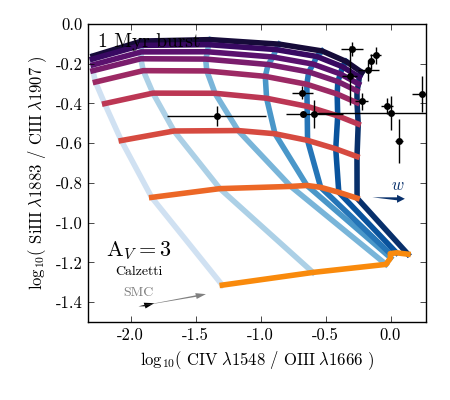
\includegraphics[width=0.45\textwidth]{figs/f16a.png}
    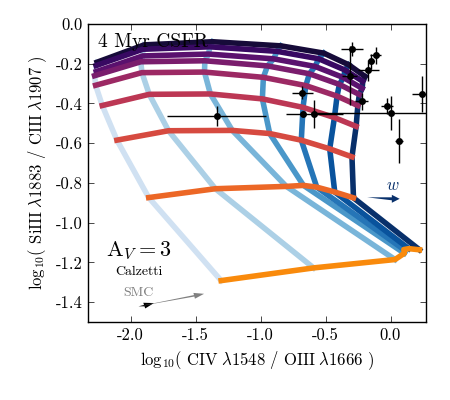
\includegraphics[width=0.45\textwidth]{figs/f16b.png}\\
    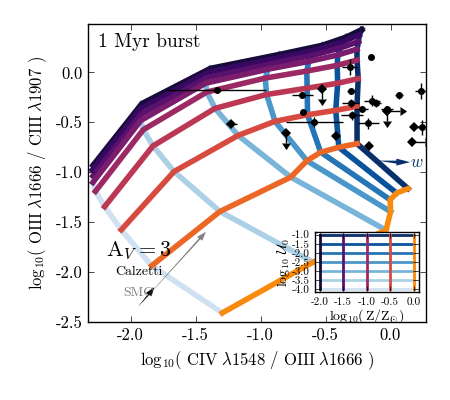
\includegraphics[width=0.45\textwidth]{figs/f16c.png}
    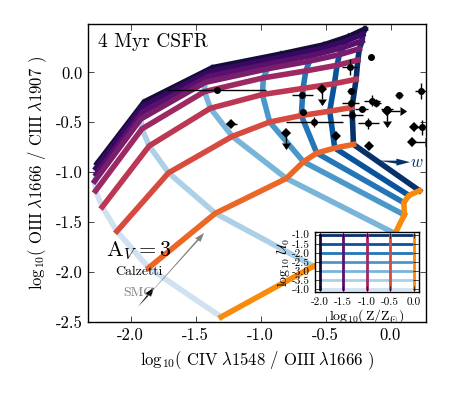
\includegraphics[width=0.45\textwidth]{figs/f16d.png}
    \caption{The \citet{Berg+2016} BCD sample compared to UV diagnostic diagrams for a 1\Myr burst (left) and a 4\Myr constant SFR (right). Observations from \citet{Senchyna+2017} are shown with grey diamonds on the bottom two plots. The blue lines connect models of constant ionization parameter. \logUeq{-1} is shown in dark blue and \logUeq{-4} is shown in light blue. Models of constant metallicity are connected by the colored lines, from \logZeq{-1} in purple and \logZeq{0.0} in yellow. Stellar wind emission can inflate the measured C\textsc{IV}1548 flux, we indicate the direction of this with the blue arrow. The grey and black arrows show three magnitudes of extinction assuming SMC and Calzetti reddening laws, respectively.}
    \label{fig:dataDD3}
  \end{center}
\end{figure*}
%-------------------------------------------------------

Contribution from both nebular emission and stellar wind emission is a known issue for other UV emission lines as well (e.g., \heii$\lambda1640$). In theory, with sufficient resolution and signal-to-noise, one could distinguish the two components by their different line profiles, as the nebular emission component should be narrow while the stellar wind emission component should be fairly broad. However, this measurement is difficult in the more common low-to-mid-resolution spectra. For this reason,  we recommend limiting diagnostic diagrams to line ratios that include no more than one emission line with a well-known stellar emission contribution. For example, the commonly used \heii$\lambda1640$ / \civ$\lambda1548$ line ratio \citep[e.g., ][]{Feltre+2016, Nakajima+2017} may be difficult to interpret due to the unknown contribution from stellar and nebular emission in both the numerator and denominator.

\subsubsection{Emission line equivalent widths} \label{sec:obs:UV:EWs}

Emission line equivalent widths (EWs) are frequently reported instead of fluxes. However, EWs are sensitive to the luminosity of the underlying continuum relative to the strength of the emission line.

To measure emission line equivalent widths from our models, we follow the methodology applied to observed data. In broad terms, the process involves subtracting the best-fit stellar continuum, and then fitting the residual emission line with a Gaussian. We generate two spectra with \FSPS, one that includes nebular emission lines and one that does not. We use the ``non-emission'' spectrum as the best-fit stellar continuum. \FSPS returns $\mathcal{F}_{\lambda}$ in \Lsun/\ang, which we convert to cgs units (erg/s/cm$^{-2}$/\ang) by assuming a total stellar mass of $M=10^7$\Msun\footnote{We chose this mass to match the observed properties of the \citet{Berg+2016} sample. However, we note that the \ciii equivalent widths presented here are not sensitive to that choice, since both the underlying UV stellar continuum and the \ciii luminosity scale directly with the flux of the same massive star population.} and a distance of 10$\,$Mpc. We subtract the continuum spectrum from the emission spectrum and fit the resultant scaled emission-line-only spectrum with \texttt{scipy.optimize.curvefit} \citep{SciPy} using a 3-parameter Gaussian function of the form:
\begin{equation}
    f(x) = a \cdot \exp \left( \frac{-(x-b)^2}{2c} \right),
\end{equation}
such that the integrated flux in the Gaussian is simply $\sqrt{2\pi} \cdot ac$ and an equivalent width with units of \ang. 

In Fig.~\ref{fig:CIIIew} we plot the model equivalent width of \ciii$\lambda\,1907,1909$ as a function of metallicity for a 1\Myr instantaneous burst, where we have added the equivalent widths of the \ciii$\lambda\,$1907 and \ciii$\lambda\,$1909.

The equivalent width of \ciii depends strongly on ionization parameter, where models with high ionization parameters produce larger \ciii equivalent widths. The equivalent widths are also strongly dependent on metallicity. The largest \ciii equivalent width (nearly 40\ang) is seen  at $\log_{10}(\mathrm{O}/\mathrm{H})\sim 8$, and declines toward both higher and lower metallicities. \ciii equivalent widths decrease much more rapidly towards high metallicities, and are essentially non-existent at solar and super-solar metallicities. \ciii equivalent widths decline to $\sim10$\ang at \logZeq{-2} due to the increasing deficit of carbon.

We compare the models in Fig.~\ref{fig:CIIIew} to measured equivalent widths and metallicities from the \citet{Berg+2016} and \citet{Senchyna+2017} samples, both of which also measure equivalent widths using single gaussian fits to the emission line. Fig.~\ref{fig:CIIIew} also includes the literature measurements compiled by \citet{Senchyna+2017}, which include nearby galaxies from \citet{Giavalisco+1996} (``G96'') and \citet{Leitherer+2011} (``L11'').

The models in Fig.~\ref{fig:CIIIew} are able to reproduce the range of observed \ciii equivalent widths and their distribution with metallicity. In particular, our models show weak \ciii equivalent widths at high metallicity ($\log_{10}(\mathrm{O}/\mathrm{H} \gtrsim 8.4$) and show the strongest \ciii equivalent widths at low metallicity ($\log_{10}(\mathrm{O}/\mathrm{H}){\sim} 8$). This behavior is in agreement with \citet{Senchyna+2017}, who suggested that there seemed to be a metallicity threshold in the observations, where large \ciii equivalent widths were only observed in galaxies with metallicities below $\log_{10}(\mathrm{O}/\mathrm{H})\sim 8.4$. Our model envelope naturally suppresses the \ciii EW at high metallicity, though perhaps not as strongly as is seen in the data.

%For galaxies with metallicities typical of present-day star forming galaxies, large \ciii equivalent widths require extreme ionization parameters (\logUeq{-1}). \ciii emission is strongest at $\log_{10}(\mathrm{O}/\mathrm{H})\sim 8$, where equivalent widths are comparable to that observed in the reionization era \citep{Stark+2015, Stark+2017}. As the gas phase metallicity continues to decrease, the \ciii equivalent widths eventually turn over to smaller values again. At the lowest metallicities in our model, we do not predict equivalent widths larger than 10-15\ang. This is likely due to the lack of available C in the gas (though see \S\ref{sec:gasZ} for a discussion variations in gas phase abundances).

%-------------------------------------------------------
% CIII equivalent widths
%-------------------------------------------------------
\begin{figure}
  \begin{center}
    \plotone{figs/f17.png}
    \caption{The equivalent width of \ciii$\lambda\,1907,1907$ as a function of metallicity for a 1\Myr instantaneous burst with $M=10^7$\Msun. The blue lines connect models of constant ionization parameter. \logUeq{-1} is shown in dark blue and \logUeq{-4} is shown in light blue. Models of constant metallicity are connected by the colored lines, from \logZeq{-1} in purple and \logZeq{0.0} in yellow. As noted in \citet{Senchyna+2017}, there seems to be a metallicity ceiling around $\log_{10}(\mathrm{O}/\mathrm{H})\sim 8$, above which \ciii emission is very weak. }
    \label{fig:CIIIew}
  \end{center}
\end{figure}
%-------------------------------------------------------

Higher ionization parameters produce larger \ciii equivalent widths at all metallicities. Thus, observations with large \ciii equivalent widths should be also biased toward high ionization parameters, and should have emission line ratios that similarly reflect that bias. We test this hypothesis in Fig.~\ref{fig:CIIIBPT}, where we show our models on optical diagnostic diagrams color-coded by their UV \ciii equivalent width. The left and middle panels show the BPT diagram and the O$_{32}$-R$_{23}$ diagram respectively. Models with large \ciii equivalent widths (redder colors) occupy the region of the BPT diagram with large values of \oiii/\hb and large ionization parameters. Similarly, the models with large \ciii equivalent widths have large O$_{32}$ ratios, also indicating high ionization parameters.

Finally, the right panel of Fig.~\ref{fig:CIIIBPT} shows the \ciii equivalent width as a function of the optical \oiii$\lambda\,5007$ equivalent width. Objects with large \oiii equivalent widths have been suggested as a means of optically selecting galaxies with strong UV \ciii emission \citep{Berg+2016, Senchyna+2017}. Our models confirm this correlation, although with an offset, due to the different metallicity dependence of carbon and oxygen line strength. The largest \ciii equivalent widths in the models do not coincide with the largest \oiii equivalent widths, since oxygen emission lines are strongest at a slightly higher metallicity ($\log_{10}(\mathrm{O}/\mathrm{H})\sim 8.4$) than the metallicity with peak \ciii emission ($\log_{10}(\mathrm{O}/\mathrm{H})\sim 8$). 

%-------------------------------------------------------
% CIII equivalent widths
%-------------------------------------------------------
\begin{figure*}
  \begin{center}
    \plotthree{figs/f18a.png}{figs/f18b.png}{figs/f18c.png}
    \caption{\emph{Left and Center:} Optical diagnostic diagrams color-coded by the equivalent width of \ciii$\lambda\,1907,1907$. Large \ciii equivalent widths occur in models with high ionization parameter, and thus coincide with observations that have large values of \oiii/\hb (\emph{left}) and large values of O3O2 (\emph{center}).  \emph{Right:} \ciii$\lambda\,1907,1907$ equivalent width as a function of \oiii$\lambda\,5007$ equivalent width. Large \ciii equivalent widths correlate with large \oiii equivalent widths.}
    \label{fig:CIIIBPT}
  \end{center}
\end{figure*}
%-------------------------------------------------------


\subsubsection{Absorption Indices} \label{sec:obs:UV:BCDs}

To evaluate the absorption line indices identified in \S\ref{sec:mod:abs}, we compare our models to measurements of 14 nearby ($0.003 < z < 0.03$) BCDs presented in \citet{Zetterlund+2015}, observed using the HST COS spectrograph. This sample has metallicities derived from optical emission line ratios from KK04 based on the R$_{23}$ diagnostic, giving an estimated accuracy of ${\sim}0.15$ dex \citep{Zetterlund+2015}. The accuracy of the R$_{23}$ metallicity diagnostic is worse near $12+\log(O/H)\sim 8.4$, where the value of R$_{23}$ rolls over, and may be biased high compared to stellar metallicities \citep[e.g.,][]{Kudritzki+2012}.

There were no nebular emission features detected in this sample, due to sample selection effects and low signal-to-noise (S/N${\sim}$1-5). However, \citet{Zetterlund+2015} did provide measurements of \texttt{AlII\_1670} and \texttt{CIV\_1550}, two of the \citet{Leitherer+2011} absorption indices.

In Fig.~\ref{fig:BCDabs} we show equivalent widths of \texttt{AlII\_1670} and \texttt{CIV\_1550} as a function of galaxy metallicity. In general, the \texttt{CIV\_1550} EWs are large, as expected for this strong, stellar-wind dominated line. The weaker \texttt{AlII\_1670} index takes both positive and negative values, potentially reflecting the influence of filling from emission lines (negative EWs), which is particularly problematic for this index, as discussed in \ref{sec:mod:abs}. 

Although some \texttt{AlII\_1670} measurements lie systematically above our model predictions, we note that our models only include the contribution from stellar and nebular emission, and do not include the effects of interstellar absorption. This was considered in detail in \citet{Vidal-Garcia+2017}, who found that interstellar line absorption near Al{\sc ii}$\lambda$1670 can be significant, especially at high metallicity. Interstellar absorption can also affect the \texttt{CIV\_1550} index, for which \citet{Leitherer+2011} noted could account for as much as 1/3 of the absorption in the index.

%-------------------------------------------------------
% Line ratio sigma
%-------------------------------------------------------
\begin{figure}
  \begin{center}
    \plotone{figs/f19.png}
    \caption{The equivalent widths of the \texttt{AlII\_1670} and \texttt{CIV\_1550} \citet{Leitherer+2011} absorption indices as a function of metallicity. The orange markers are measured from local BCD spectra, with metallicity estimates derived from optical emission line ratios. The blue lines show our emission model at several different ionization parameters for a 4\Myr CSFR.}
    \label{fig:BCDabs}
  \end{center}
\end{figure}
%-------------------------------------------------------

In addition to the effects from interstellar absorption, the central bandpass of the \texttt{AlII\_1670} index also includes the \alII$\lambda1670$ emission line. We briefly estimate the total possible contribution from nebular emission to the absorption indices shown in Fig.~\ref{fig:BCDabs}. Models that include nebular emission predict equivalent widths $0.1 - 0.5$ \ang smaller than the stellar-only predictions; this contribution can be significant, however, since typical \texttt{AlII\_1670} EWs are of order 0.5\ang. 

Similarly, the central bandpass of the \texttt{CIV\_1550} absorption index includes the \civ$\lambda1548$ emission line. However, \texttt{CIV\_1550} is less susceptible to nebular influence since the stellar wind absorption feature that dominates the central bandpass has equivalent widths of order 5-10\ang, whereas the nebular emission contributes 0.01\ang at most to the total equivalent width, which is entirely negligible compared to the measured errors.

\subsection{UV spectra of high redshift galaxies} \label{sec:obs:UV:LBGs}

Rest-frame UV spectra of distant galaxies are a powerful tool to study the star formation environment of young galaxies, and will become higher quality and increasingly commonplace with future optical and IR instruments on the next generation of telescopes. In this section we compare the UV diagnostic diagrams presented in \S\ref{sec:mod:comb} to the rest-frame UV spectra of galaxies at intermediate- and high-redshift obtained with ground-based optical and IR instruments.

Before proceeding, we note that that estimates of metallicity for these distant galaxies, when used, are determined from rest-frame optical emission line diagnostics observed in the IR. These diagnostics are calibrated against local galaxies, where the star forming environment could be drastically different from the star forming environment typical of distant galaxies, and for which the application of local metallicity diagnostics may not be appropriate. It is still interesting, however, to understand where and why the emission line models succeed or fail; to that end, we compare our model to as many observations of galaxies between redshifts 1 and 3 as possible.

%-------------------------------------------------------
% logZ line ratio
%-------------------------------------------------------
\begin{figure*}
  \begin{center}
    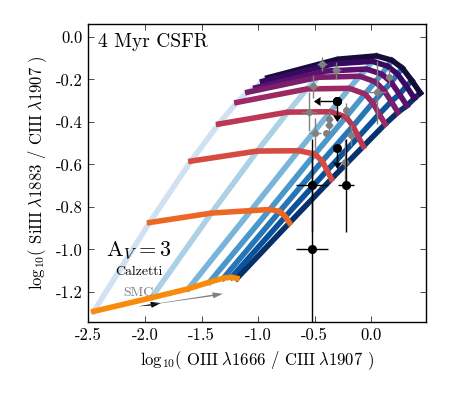
\includegraphics[width=0.45\textwidth]{figs/f20a.png}
    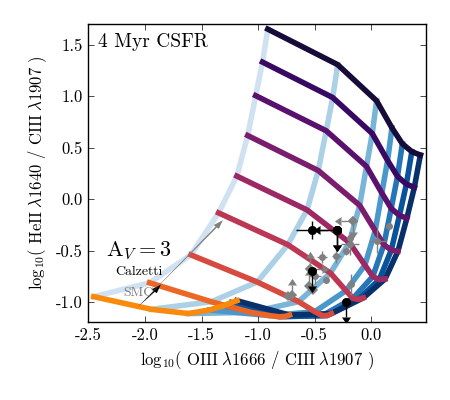
\includegraphics[width=0.45\textwidth]{figs/f20b.png}\\
    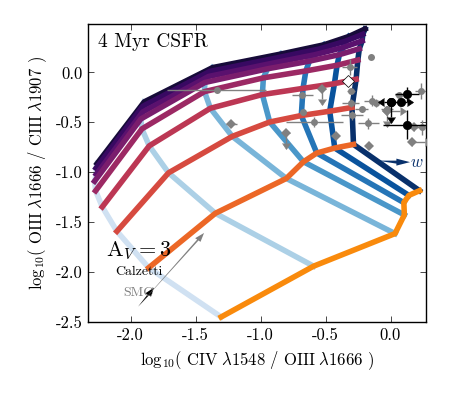
\includegraphics[width=0.45\textwidth]{figs/f20c.png}
    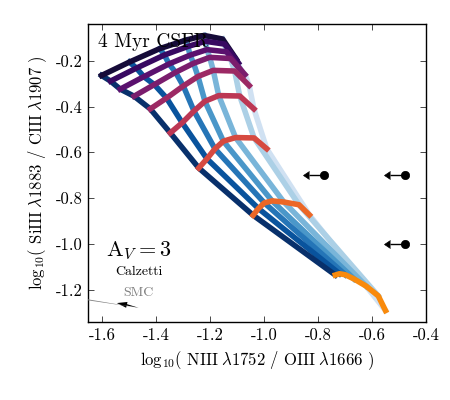
\includegraphics[width=0.45\textwidth]{figs/f20d.png}
    \caption{The \citet{Stark+2014} galaxies at $z{\sim}2$ (solid black circles) compared to UV diagnostic diagrams assuming a 4\Myr stellar population with constant SFR. The blue lines connect models of constant ionization parameter. \logUeq{-1} is shown in dark blue and \logUeq{-4} is shown in light blue. Models of constant metallicity are connected by the colored lines, from \logZeq{-1} in purple and \logZeq{0.0} in yellow. The \citet{Berg+2016} local BCD sample (grey circles) is included in the upper left, upper right, and lower left diagrams; the \citet{Senchyna+2017} local BCD sample (grey diamonds) is included in the lower left diagram. Stellar wind emission can inflate the measured C\textsc{IV}1548 flux, we indicate the direction of this with the blue arrow. The grey and black arrows show three magnitudes of extinction assuming SMC and Calzetti reddening laws, respectively.}
    \label{fig:dataHiZ}
  \end{center}
\end{figure*}
%-------------------------------------------------------

In Fig.~\ref{fig:dataHiZ}, we show several diagnostic diagrams with a sample of intermediate and high redshift galaxies compiled from \citet{Stark+2014} (black circles) and \citet{Christensen+2012} (white diamond). The \civ$\lambda1548$, \SiuIII$\lambda1883$, \oiii$\lambda1666$, \ciii$\lambda1906$ emission lines are measured in both the local galaxy sample from \citet{Berg+2016} and the lensed $z{\sim}3$ galaxy sample from \citet{Stark+2014}. We include the local galaxy observations in Fig.~\ref{fig:dataHiZ} as grey circles. \citet{Stark+2015} provides lower limits on the \SiuIII$\lambda1883$ emission line in cases where it was not detected based on observational limits.

In the Si3C3 \vs O3C3 diagram in Fig.~\ref{fig:dataHiZ} (\emph{upper left}), all of the high redshift galaxies have emission line ratios consistent with the model predictions. Overall, the line ratios for the high redshift galaxies tend toward higher ionization parameters and slightly higher metallicities than the local sample. This trend is likely driven entirely by the strength of the \ciii line, which is notably large in many of the high redshift galaxies \citep{Stark+2014}, but variations in \SiuIII$\lambda1883$ (an $\alpha$-element) could also play a role. Again, the shift towards higher ionization parameters and higher metallicities in the high redshift sample compared to local BCDs is not unexpected, given the bias toward more massive, high SFR galaxies in the former.

We show \heii$\lambda$1640/\ciii$\lambda$1907 ratio (He2C3) \vs the \oiii$\lambda$1666/\ciii$\lambda$1907 ratio (O3C3) in the upper right panel of Fig.~\ref{fig:dataHiZ}. All of the high redshift galaxies have emission line ratios consistent with the model predictions. The high redshift galaxies and the local galaxies occupy similar regions of the diagram, with no clear offset in metallicity or ionization parameter. However, all of the observations lie near models with higher metallicities than in previous diagnostic diagrams. The He2C3 ratio uses emission lines more widely spaced in wavelength than the other ratios in Fig.~\ref{fig:dataHiZ}, which could indicate that reddening corrections are responsible for the shift.

In the C4O3 \vs O3C3 diagram in Fig.~\ref{fig:dataHiZ} (\emph{lower left}), the high redshift galaxies occupy a region entirely beyond the model grid with large values of C4O3. The range of observed C4O3 and O3C3 values in the high redshift galaxies are consistent with values observed in the local galaxy sample from \citet{Berg+2016} and \citet{Senchyna+2017}, though the local sample extends to lower values of C4O3 and has a wider range in O3C3. These differences are not entirely unexpected, since the high redshift sample is smaller and necessarily probes the brightest observable targets. The high C4O3 ratios observed in the high redshift sample may support the idea that high redshift galaxies have on average ``harder'' ionizing spectra. Though we again note the important contribution stellar winds make to the C4O3 ratio, as noted by the blue arrow and discussed in \S\ref{sec:obs:UV:BCDs} (Fig.~\ref{fig:dataDD3}).

The N\textsc{ii}]$\lambda1750,1752$ emission doublet was not detected in any of the \citet{Stark+2014} sample, but lower limits were provided based on observational constraints. Despite the current non-detection, with more sensitive facilities the N\textsc{ii}]$\lambda1750$ / O\textsc{iii}]$\lambda1666$ line ratio (N2O3) could become a promising diagnostic when paired with Si3C3, which we show in the bottom right panel of Fig.~\ref{fig:dataHiZ}.
%% 
%%%%%%%%%%%%%%%%%%%%%%%%%%%%%%%%%%%%%%%%%%%%%%%%%%%%%%%%%%%%%%%%%%%%%%%%%%%%%%%%
%% 
\section{Metallicity and abundance complications} \label{sec:gasZ}

In the previous sections, we used the abundances specified in \S\ref{sec:model:neb} and assumed that the gas phase abundances track the stellar metallicity closely. In the early universe, however, these assumptions may not be appropriate in all cases. To explore this possibility, in this section, we modify the gas phase abundances from our original prescription and explore the resultant changes in emission line properties. We begin with a discussion of important gas coolants, carbon and nitrogen, before discussing more general implications of elemental abundance patterns.

\subsection{Sensitivity to C/O prescription} \label{sec:gasZ:CO}

Photoionization models must make various assumptions about the relative gas phase abundances of different elements. In general, nebular models assume that the abundances of all elements increase linearly with increasing metallicity. Specific choices are usually motivated by the desire to match the observed properties of samples of \hii regions. Most emission line strengths will depend linearly on their elemental abundances, to first order, but variations in important gas coolants like C, N, and O have additional effects on the \hii region structure and temperature, which in turn complicates the response of emission lines to changes in their abundances.

The treatment of relative elemental abundances is further complicated by the likelihood that both C and N scale non-linearly with metallicity. Nitrogen has known secondary nucleosynthetic production at high metallicity, wherein nitrogen is dredged up during the bottleneck step of the CNO cycle, which is directly dependent on metallicity. In the case of carbon, the triple-$\alpha$ process is the only known production process, but it does not depend on metallicity. Instead, additional carbon is produced through metallicity-dependent processes such as stellar winds, rather than a nucleosynthetic process. Thus, carbon is said to have a ``pseudo-secondary'' production process.

Nitrogen abundances are relatively easy to determine for local galaxies with optical spectra, and the relationship between N/O with metallicity has been well-studied \citep[e.g.,][]{Garnett+1990, vanZee+1998, Berg+2012}. Based on existing data, most photoionization models adopt a functional form for the relationship between the oxygen abundance and the N/O ratio that matches observations of local dwarf galaxies, massive extragalactic \hii regions, and starburst nucleus galaxies.

The C/O relationship is particularly relevant to this work, since \ciii is one of the strongest emission lines in the UV and is included in many of the emission line diagnostics presented in this work. Historically, carbon has been a difficult element to derive absolute abundances for, since few strong transitions exist in the optical or IR, and the optical recombination lines (RLs) become too faint to detect below $12+\log(O/H)=8$ \citep{Esteban+2014}.

Recently, \citet{Berg+2016} analyzed the relationship of C/O with metallicity in low-metallicity galaxies using collisionally-excited lines (CELs) for C and O in the UV. \citet{Berg+2016} found that the C/O ratio was roughly constant across the metallicity range of their sample ($7<12+\log(O/H)<8$). However, when combined with C/O measurements based on optical recombination lines from galaxies at higher metallicities, C/O appears to increase with metallicity above $12+\log(O/H)=8$. These data are shown in the right panel of Fig.~\ref{fig:CNO}.
%Berg 16 actually says that we cannot distinguish between an increasing relationship or a flat relationship for 12+log(O/H) < 8. With our new data, this is further cemented. The relationship appears fairly flat, with lots of scatter. Then the C/N trend makes sense, because N/O is also flat (primary only) at 12+log(O/H) < 8.

In Fig.~\ref{fig:CNO}, we show the existing N/O (\emph{left}) and C/O (\emph{right}) measurements along with the relationships between N/O and C/O used here and in various other nebular models. For both N/O and C/O, we have modified the \citet{Dopita+2013} prescription such that it plateaus for $12+\log[ O/H ] \lesssim 8$ to better match observations. The exact functional form is given in Eqs.~\ref{eq:nitrogen} \& \ref{eq:carbon} in \S\ref{sec:model:neb}, and shown as the blue line in Fig.~\ref{fig:CNO}. As noted in \citet{Steidel+2014}, the precise behavior of the N/O ratio with metallicity depends on the calibration sample and the details of the methods used to measure the abundances, and unsurprisingly there is a substantial range in the N/O versus O/H relationships applied in recent literature.

%-------------------------------------------------------
% CNO
%-------------------------------------------------------
\begin{figure*}
  \begin{center}
    \plotone{figs/f21.png}
    \caption{\emph{Left:} N/O relationships used by different nebular models. The dark and light blue points are from \citet{Berg+2016} and \citet{Berg+2012}, respectively. The grey points are massive extragalactic \hii regions from \citet{vanZee+1998}, used to calibrate the \citet{Dopita+2013} and \citet{Dopita+2000} models. The teal points are from \citet{Contini+2002}, part of the calibration sample used by \citet{Gutkin+2016}. \emph{Right:} C/O relationships used by different nebular models. The blue points are from \citet{Berg+2016}, with C/O abundances derived from UV collisionally excited lines. The teal points are extragalactic recombination line estimates from \citet{Esteban+2014}. The gold star in both plots represents where the Sun would be located according to the \citet{Asplund+2009} solar abundance set.}
    \label{fig:CNO}
  \end{center}
\end{figure*}
%-------------------------------------------------------

%The equations used in this work to model the relationship between [N/H] and [O/H] and [C/H] and [O/H] (Eq.~\ref{eq:carbon} in \S\ref{sec:model:neb}) is derived to better match the observations presented in \citet{Berg+2016}. We favor this sample for two main reasons. First, because this work focuses on UV emission line diagnostics and \citet{Berg+2016} has assembled the most comprehensive picture of UV-based C/O determinations to date, by combining their new observations with literature measurements. Second, because the chemical abundances and physical conditions for the \citet{Berg+2016} sample are all derived in a uniform, consistent manner. We have found that including a pseudo-secondary nucleosynthetic contribution for [C/H] is necessary to reproduce UV emission line observations of galaxies.

The behavior of both the N/O and C/O ratio are important for the UV emission line diagnostics presented in this work. In Fig.~\ref{fig:COvarA} we show how the \ciii$\lambda$1907 emission line changes while varying C/O at constant oxygen abundance. The left panel of Fig.~\ref{fig:COvarA} demonstrates that at constant $12 + \log (\mathrm{O}/\mathrm{H})$, while \ciii$\lambda$1907 emission depends strongly on ionization parameter (varying from $10^{32}$ to $10^{36}$ergs$\cdot$s$^{-1}$), the strength of the line is essentially independent of the actual carbon abundance. 

%Perhaps surprisingly, despite the order of magnitude decrease in carbon abundance there is no significant decrease in emission line strength. From the right panel of Fig.~\ref{fig:COvarA}, for a fixed number of ionizing photons, \ciii has a weak dependence on density, consistent with other photoionization studies of \ciii emission using \Cloudy \citep[e.g.,][]{Jaskot+2016, Feltre+2016}

While \ciii$\lambda$1907 is not a direct measure of the carbon abundance on its own, when \ciii$\lambda$1907 is paired with \oiii$\lambda$1666 it becomes much more sensitive to the relative abundance of carbon. Fig.\ref{fig:COvarB} shows the \oiii/\ciii emission line ratio as a function of ionization parameter and carbon abundance at constant $12 + \log_{10} (\mathrm{O}/\mathrm{H})$. The decreasing abundance of carbon ultimately inhibits cloud cooling, which raises the temperature of the nebula slightly and produces variations in oxygen line strength at constant $12 + \log_{10} (\mathrm{O}/\mathrm{H})$. The O3C3 line ratio is very sensitive to ionization parameter and the C/O ratio while being relatively insensitive to gas density.
%-------------------------------------------------------
% CO variation 1
%-------------------------------------------------------
\begin{figure*}
  \begin{center}
    \plottwo{figs/f22a.png}{figs/f22b.png}%\\
    %\plottwo{figs/f22c.png}{figs/f22d.png}
    \caption{The variation in \ciii$\lambda1907$ line strength as a function of ionization parameter as the abundance of C is changed at constant $12+\log_{10}(\mathrm{O}/\mathrm{H})$ abundance for a 4\Myr CSFR model at solar (\emph{left}) and 10\% solar (\emph{right}) metallicity. \ciii is sensitive to ionization parameter and moderately sensitive to gas density. \ciii is sensitive to the overall gas phase metallicity; at fixed oxygen abundance, a two order of magnitude change in carbon abundance produces relatively little variation in line strength.}
    \label{fig:COvarA}
  \end{center}
\end{figure*}
%-------------------------------------------------------

%-------------------------------------------------------
% CO variation 2
%-------------------------------------------------------
\begin{figure*}
  \begin{center}
    \plottwo{figs/f23a.png}{figs/f23b.png}%\\
    %\plottwo{figs/f23c.png}{figs/f23d.png}
    \caption{The variation in the \oiii$\lambda1666$/\ciii$\lambda1907$ (O3C3) emission line ratio as a function of ionization parameter as the abundance of C is decreased at constant $12+\log[O/H]$ abundance for a 4\Myr CSFR model at solar (\emph{left}) and 10\% solar (\emph{right}) metallicity. The decrease in C abundance inhibits cloud cooling, raising the temperature of the nebula slightly, producing variations in oxygen line strength at constant $12+\log[O/H]$. The O3C3 line ratio is very sensitive to ionization parameter, metallicity, and the C/O ratio.}
    \label{fig:COvarB}
  \end{center}
\end{figure*}
%-------------------------------------------------------

Despite our modifications to previous abundance prescriptions, our nebular model still produces BPT diagram line ratios that are consistent with observations. In Fig.~\ref{fig:BPT1} we show model grids on BPT diagrams assuming the four different abundance prescriptions considered in Fig.~\ref{fig:CNO}: the abundance prescription used in this work, the \citet{Dopita+2013} prescription (``D13''), the \citet{Dopita+2000} prescription (``D00''), and the \citet{Gutkin+2016} abundance prescription (``G16''). The models are run for identical input parameters and the only modification is the mixture of gas-phase abundances specified in \Cloudy. However, the resultant model grids vary by 0.4 dex in \nii/\ha.

The model presented here is able to reproduce the star-forming sequence quite well, while simultaneously producing UV emission line ratios consistent with observed galaxies. The other abundance prescriptions struggle with this: the \citet{Dopita+2013} nitrogen abundances are too low to correctly reproduce the optical star-forming sequence, though they do well at predicting the UV \ciii behavior. The \citet{Dopita+2000} model is able to reproduce the optical star-forming sequence, but does not include the additional pseudo-secondary contribution for carbon needed to explain the UV observations.

We note that Fig.~\ref{fig:BPT1} is only intended to highlight how changes in the adopted relative elemental abundances can change emission line ratio predictions. The behavior displayed in Fig.~\ref{fig:BPT1} is not representative of the other models' ability to reproduce observed line ratios, as each of these models can and does adequately reproduce the locus of star-forming galaxies through adopting different physical parameters than that used in \CloudyFSPS. The grids shown in Fig.~\ref{fig:BPT1} use the elemental abundance prescriptions from the above models, but are all run using the specific combination of input parameters chosen for the \CloudyFSPS nebular model.

This reflects the particular strengths of the different nebular models. The \citet{Dopita+2013} models allow users to make use of different, non-Maxwellian electron velocity distributions in the nebula. The \citet{Gutkin+2016} model is unique in that by design it does \emph{not} fix the C and N abundances to solar-scaled values and allows them to be varied to produce arbitrary C/O and N/O ratios. This makes their model uniquely qualified to understand the behavior of C/O and N/O ``outliers''.

We show the model grids with different abundances on alternative emission line diagnostic diagrams in Fig.~\ref{fig:BPT2} and Fig.~\ref{fig:BPT3} to highlight how the different abundance prescriptions change the model grid. The abundance prescription used in this work produces optical line ratios that are well-matched with observed galaxies. To show where observed galaxies lie in each of these diagnostic diagrams, we include a 2D histogram showing the number density of star forming galaxies, as done in \citet{Byler+2016}. The star-forming galaxy sample is derived from galaxy spectra from the Sloan Digital Sky Survey Data Release 7 \citep[SDSS DR7;][]{York+2000, Abazajian+2009} and emission line fluxes measured from the publicly available SDSS DR7 MPA/JHU catalog \citep{Kauffmann+2003a, Brinchmann+2004, Salim+2007}. We use the emission line sample presented in \citet{Telford+2016}, briefly summarized here. The sample includes $\sim 135,000$ galaxies with redshifts between 0.07 and 0.30. Galaxies are required to have S/N of 25 in the \ha{} line, 5 in the \hb{} line, and 3 in the \sii{} lines. Emission line fluxes are corrected for dust extinction using the Balmer decrement and the \citet{Cardelli+1989} extinction law, assuming $R_{\mathrm{V}} = 3.1$ and an intrinsic Balmer decrement of 2.86. AGNs are removed from the sample according to the empirical BPT diagram classification of \citet{Kauffmann+2003b}.

%-------------------------------------------------------
% BPT Diagrams
%-------------------------------------------------------
\begin{figure}
  \begin{center}
    \plotone{figs/f24.png}
    \caption{Model grids on the standard BPT diagram. The greyscale 2D histogram shows the number density of SDSS star-forming galaxies from the \citet{Telford+2016} sample. All models assume a 1 Myr instantaneous burst and otherwise identical input parameters. Each panel represents a model run with a different abundance prescription, as noted in the upper right corner of each plot, and shown in Fig.~\ref{fig:CNO}. Changing the behavior of the N/O ratio relative to solar at a given [O/H] shifts the \nii/\ha emission line ratio and the location of the models in a BPT diagram.}
    \label{fig:BPT1}
  \end{center}
\end{figure}
%-------------------------------------------------------
\begin{figure}
  \begin{center}
    \plotone{figs/f25.png}
    \caption{Model grids on a diagnostic diagram. The greyscale 2D histogram shows the number density of SDSS star-forming galaxies from the \citet{Telford+2016} sample. All models assume a 1 Myr instantaneous burst and otherwise identical input parameters. Each panel represents a model run with a different abundance prescription, as noted in the upper right corner of each plot, and shown in Fig.~\ref{fig:CNO}.}
    \label{fig:BPT2}
  \end{center}
\end{figure}
%-------------------------------------------------------
\begin{figure}
  \begin{center}
    \plotone{figs/f26.png}
    \caption{Model grids on a diagnostic diagram. The greyscale 2D histogram shows the number density of SDSS star-forming galaxies from the \citet{Telford+2016} sample. All models assume a 1 Myr instantaneous burst and otherwise identical input parameters. Each panel represents a model run with a different abundance prescription, as noted in the upper right corner of each plot, and shown in Fig.~\ref{fig:CNO}.}
    \label{fig:BPT3}
  \end{center}
\end{figure}
%-------------------------------------------------------


\subsection{Decoupled gas and stellar metallicities}

Our models assume that the massive stars that dominate the UV stellar continuum have the same metallicity and abundance pattern as the gas that they ionize. However, there are scenarios in which it is possible that the gas phase abundances differ from the stellar abundances. These include the injection of metal-enriched gas from stellar outflows or the rapid accretion of metal-poor gas during fueling of a star formation event. The latter of these would likely be most important during early epochs of star formation, with high gas inflow rates, which would be required for accretion to dilute the gas on $<10$\Myr timescales. Early star formation could also take place in gas enriched in $\alpha$-elements, due to the reduced fraction of Type Ia supernovae (SNe).

Recently, \citet{Steidel+2016} have suggested that the stellar and gas phase abundances should be decoupled due to the $\alpha$ enhancement of the gas relative to the stellar population. In their scenario, to first order, the stellar metallicity will follow the iron abundances while the gas metallicity should follow the measured oxygen abundances. From Salpeter IMF-averaged yields for O/Fe based on core collapse supernovae, \citet{Steidel+2016} estimates that this could produce nebular oxygen abundances that are 4-5 times larger than the stellar Fe-based metallicity. 

We have generated models where both the gas and stellar abundances are allowed to vary to explore the observable consequences of this choice.

We cannot self-consistently model $\alpha-$enhanced gas, since the MIST models used in this work for the stellar ionizing spectrum rely on solar-scaled abundances. To mimick the effects of $\alpha-$enhancement, we thus decouple the stellar metallicity from the gas phase metallicity and allow the relative gas phase abundances to increase above the stellar abundances. This will ``enhance'' the gas in $\alpha$-elements like O, Mg, Al, Ti, and Si, but will also enhance Fe-peak elements in the gas. We do not expect this to change the results qualitatively, since Fe does not play a large role in determining the thermodynamics of the gas. 

We first model the ``enriched gas'' scenario by pairing a low-metallicity SSP (\logZeq{-1}) with moderate metallicity gas (\logZeq{-0.5}). These values are motivated by \citet{Steidel+2016}, who found that abundance determinations sensitive to stellar photospheric line blanketing features gave a metallicity of \logZeq{-1} while nebular emission lines, primarily optical oxygen and nitrogen lines, gave a metallicity of \logZeq{-0.4}, or Z$_{\mathrm{gas}}$ = $4\,$Z$_{\mathrm{star}}$.

%-------------------------------------------------------
% diffZ BPT
%-------------------------------------------------------
\begin{figure*}
  \begin{center}
    \plotthree{figs/f27a.png}{figs/f27b.png}{figs/f27c.png}
    \caption{Impact of varying the gas phase metallicity (Z$_{\mathrm{gas}}$) for a fixed stellar metallicity (Z$_{\mathrm{star}}$; \logZeq{-1}). \emph{Left:} The standard BPT diagram. The blue lines show a standard model grid varying in ionization parameter and metallicity, where Z$_{\mathrm{gas}}$ = Z$_{\mathrm{star}}$. The markers show the models where Z$_{\mathrm{gas}}$ is decoupled from Z$_{\mathrm{star}}$.  All model points assume the same ionizing spectrum: a stellar population with constant SFR over 4\Myr and $\log_{10} \mathrm{Z}_{\mathrm{star}}/\mathrm{Z}_{\odot} = -1$. The color of the markers represent models with different ionization parameters. The circular marker shows the location where the gas phase metallicity equals the stellar metallicity, Z$_{\mathrm{gas}}=$Z$_{\mathrm{star}}$. The star-shaped marker shows the ``enriched model'' (\logZeq{-0.5}; Z$_{\mathrm{gas}}=3\,$Z$_{\mathrm{star}}$). \emph{Center \& Right:} The \nii/\ha (\emph{center}) and \oiii/\hb (\emph{right}) line ratios as a function of Z$_{\mathrm{gas}}$ and ionization parameter. The dashed line indicates where $\mathrm{Z}_{\mathrm{gas}}=\mathrm{Z}_{\mathrm{star}}$. Both line ratios increase as the gas metallicity is enhanced.}
    \label{fig:diffZ}
  \end{center}
\end{figure*}
%-------------------------------------------------------

We show the models with decoupled gas and stellar metallicities in Fig.~\ref{fig:diffZ}. These decoupled models reflect responses to gas inflow or localized enrichment with the same abundance pattern, or alternatively, can reflect abundance differences between the gas and stars in part due to the different elements that dominate the ISM cooling and emission lines and the stellar atmosphere.

For a fixed ionizing spectrum, an enhanced gas phase metallicity shifts line ratios to larger \nii/\ha and \oiii/\hb ratios by ${\sim}1\,$dex at all ionization parameters. This shift occurs because the metal-poor ionizing spectrum is harder and provides more ionizing photons, while the gas enriched in N and O produces larger BPT line ratios. This shift would be consistent with observations of galaxies at high redshift, which show extreme BPT line ratios, particularly at high \oiii/\ha.  Decoupling the gas and stellar metallicities is thus an enticing explanation for the optical emission lines.

Unlike the optical, where \oiii is one of the strongest optical emission lines, the \ciii$\lambda\lambda$1907,9 doublet is the strongest UV emission line after Ly$\alpha$. In Fig.~\ref{fig:diffZCO} we show how \ciii$\lambda$1907 emission responds to a change in gas phase metallicity for a fixed stellar metallicity of \logZeq{-1}. \ciii$\lambda$1907 is very sensitive to ionization parameter and weak at high metallicities. In an enriched gas model (Z$_{\mathrm{gas}}$ $>$ Z$_{\mathrm{star}}$) we would expect \ciii$\lambda$1907 to be weaker and the ratio of \oiii$\lambda$1666/\ciii$\lambda$1907 to be weaker. This is in conflict with observations, which show strong \ciii$\lambda$1907 emission and strong \oiii$\lambda$1666/\ciii$\lambda$1907 ratios, implying gas phase oxygen abundances at or below $12+\log_{10}(\mathrm{O}/\mathrm{H})\sim 8$. Explaining the extreme \oiii/\ha ratios and \ciii emission in objects at high redshift may require a combination of $\alpha$-enhancement and elevated N/O abundances. 

%-------------------------------------------------------
% diffZ CIII
%-------------------------------------------------------
\begin{figure*}
  \begin{center}
    \plottwo{figs/f28a.png}{figs/f28b.png}
    \caption{Changes in the \oiii/\ciii ratio from varying the gas phase abundances (Z$_{\mathrm{gas}}$) at fixed stellar metallicity (Z$_{\mathrm{star}}$; \logZeq{-1}). The dashed line indicates where the stellar and gas phase metallicities are equal. Unlike the BPT line ratios shown in Fig.~\ref{fig:diffZ}, which increase as $\mathrm{Z}_{\mathrm{gas}}$ gets larger than $\mathrm{Z}_{\mathrm{star}}$, the \oiii/\ciii ratio is largest when $\mathrm{Z}_{\mathrm{gas}}\lesssim \mathrm{Z}_{\mathrm{star}}$.}
    \label{fig:diffZCO}
  \end{center}
\end{figure*}
%-------------------------------------------------------


%% 
%%%%%%%%%%%%%%%%%%%%%%%%%%%%%%%%%%%%%%%%%%%%%%%%%%%%%%%%%%%%%%%%%%%%%%%%%%%%%%%%
%% 
\section{Feasibility Estimates} \label{sec:feas}

In this section we discuss the feasibility of measuring important UV lines with existing and planned observatories. We quantify the utility of the diagnostics from \S\ref{sec:obs} with the launch of JWST, which will provide rest-frame UV spectra of galaxies at $z \geq 4$, and we identify potential diagnostics for the redshift ranges probed by the JWST spectrograph.

In Fig.~\ref{fig:jwst}, we show observable UV emission lines as a function of the desired redshift range to be probed with JWST. Each emission line is color-coded by its strength relative to \hb for a fiducial model assuming a 4\Myr constant SFR, \logUeq{-2.5} and \logZeq{-0.5}, so users can determine the brightest emission lines in their desired redshift range. We also highlight the range of redshifts where each of the emission line ratios presented in Table~\ref{tab:ratios} are observable.

%-------------------------------------------------------
% JWST
%-------------------------------------------------------
\begin{figure*}
  \begin{center}
    \plotone{figs/f29.png}
    \caption{We show the relevant redshift ranges observable with JWST's NIRSpec instrument with the G140 grating. Each line is color-coded by its luminosity compared to the luminosity of \hb, assuming a 4\Myr constant SFR population with \logZeq{-0.5} and \logUeq{-2.5}.}
    \label{fig:jwst}
  \end{center}
\end{figure*}

%-------------------------------------------------------
For the highest redshift galaxies expected to be discovered with JWST, $7 < z < 10$, low-resolution spectroscopy ($R\sim10-100$) can be obtained with NIRSpec \citep{Levesque+2015n}, allowing for the detection of the brightest emission lines like \ciii$\lambda\,1906,1909$ and \oiii$\lambda\,1661,1666$. In this regime, the O3C3 emission line ratio and the slope of the UV continuum are likely to be the most useful probes of the ISM properties.

For galaxies between $5 < z < 7$, NIRSpec will provide mid-resolution ($R\sim1000$) spectroscopy for reasonable exposure times. This is high enough resolution to employ most of the diagnostic diagrams presented in this work, including O3C3, Si3C3, S3C3, Si3N3, S3O3, and N3O3. These diagnostics are sensitive to ionization, metallicity, and the underlying stellar population, which we can use to understand and distinguish the ISM properties of galaxies during the epoch of their formation.

For a smaller subset of galaxies, high-resolution ($R\sim2700$) spectra can be obtained. These spectra will be able to resolve stellar absorption features, enabling the simultaneous study of the nebular emission and stellar population. In this regime, the diagnostics combining emission and absorption features will provide insight into the conversion of gas into stars, stellar feedback and chemical enrichment.

%% 
%%%%%%%%%%%%%%%%%%%%%%%%%%%%%%%%%%%%%%%%%%%%%%%%%%%%%%%%%%%%%%%%%%%%%%%%%%%%%%%%
%% 
\section{Conclusions} \label{sec:conclusions}
We build upon the nebular model framework established in \citet{Byler+2016}, extending the self-consistent predictions for nebular line and continuum emission from stellar populations into the UV regime. Our conclusions are as follows:

\begin{itemize}
    \item We have identified UV emission lines that are bright and correlate strongly with bulk physical properties of the nebula like the gas phase metallicity and the hardness and intensity of the ionizing spectrum. We provide predicted UV emission line fluxes as a function of metallicity and ionization parameter in a machine-readable format.
    \item We distinguish combinations of emission lines that will be useful diagnostics for bulk properties like metallicity and ionization parameter. These emission line ratios are bright, relatively insensitive to reddening, and correlate with metallicity and ionization parameter.
    \item Unlike the optical portion of the spectrum, the stellar continuum in the UV is dominated by the same stars that are responsible for producing the ionizing radiation that drives nebular emission. We gain additional metallicity leverage by considering stellar absorption features as diagnostics. We determine which of the absorption line indices presented by \citet{Leitherer+2011} are the most useful metallicity diagnostics and quantify the contribution from nebular emission to each absorption index.
    \item The metallicity of the short-lived massive stars that produce the UV continuum should be nearly identical to that of the surrounding nebula. The joint analysis of stellar and nebular features leverages our model's ability to self-consistently link the temporal and metallicity dependent changes in the stellar absorption features to the nebular emission lines. We identify combinations of stellar absorption features and nebular emission lines that can be used as metallicity and ionization parameter diagnostics.
    \item We evaluate the emission and absorption diagnostics by comparing them with observed galaxies. We confirm that the diagnostics can reproduce observed emission and absorption from a sample of local BCDs. For line ratios where the contribution from stellar wind emission plays a role in one of the emission lines (e.g., \civ or \heii), the model predictions are unable to fully reproduce observations. We advise caution when interpreting line ratios where both emission lines could include a significant contribution from stellar winds, like \civ/\heii. 
    \item We verify that the diagnostics hold across redshift by comparing them with observations of high redshift galaxies. In general, the model grids are consistent within errors of high redshift observations.
    \item We explore the repercussions of decoupling the stellar metallicity from the gas phase metallicity. Pairing an ionizing spectrum for a metal-poor stellar population with gas enriched in N and O produces BPT line ratios that are 3 dex larger than if the metal-poor population was paired with similarly metal-poor gas. This may help explain the observations of objects at high redshift with ``extreme'' \oiii/\ha ratios. However, this explanation does not hold for extreme \ciii emission, which is strongest when the stars and gas are similarly metal-poor.
    \item We discuss the importance of the relative elemental abundance prescriptions used in photoionization models. In particular, the applied relationship between nitrogen and carbon with metallicity ultimately dictates the model's ability to reproduce observed emission line ratios in various diagnostic diagrams. We apply relationships that specify the behavior of [N/H] and [C/H] with [O/H] that are designed to better match observed galaxies. Our model is able to simultaneously reproduce observed UV \emph{and} optical emission line ratios, including the standard BPT diagram and its most common variants.
    \item We recommend diagnostics for the redshift ranges probed by the JWST spectrograph. The mid-resolution ($R\sim1000$) spectroscopy that NIRSpec will provide for galaxies between $5 < z < 7$ is ideal for the use of the emission line diagnostics presented here, including O3C3, Si3C3, S3C3, Si3N3, S3O3, and N3O3. 
\end{itemize}

\acknowledgments

It is a pleasure to thank Grace Telford and Claus Leitherer for helpful discussions informing the ideas presented here. Special thanks to JJ Eldridge, Mason Ng, and Georgie Taylor for sharing with us unpublished WMBasic models (Eldridge et al., in prep); to Erika Zetterlund and Charles Danforth for sharing with us the reduced spectra from \citet{Zetterlund+2015}; and to Danielle Berg, for sharing with us unpublished emission line measurements (Berg et al., in prep). C.C. acknowledges support from NASA grant NNX13AI46G, NSF grant AST- 1313280, and the Packard Foundation. N.B. acknowledges support from the University of Washington's Royalty Research Fund Grant 65-8055.
%We would also like to thank the anonymous referee for thorough and constructive feedback that greatly improved the paper.
\software{astropy \citep{Astropy},  
          Cloudy \citep{Ferland+2013},
          cloudyFSPS \citep{cloudyFSPSv1},
          FSPS \citep{Conroy+2009, Conroy+2010},
          python-fsps \citep{pythonFSPSdfm}} 

%% 
%%%%%%%%%%%%%%%%%%%%%%%%%%%%%%%%%%%%%%%%%%%%%%%%%%%%%%%%%%%%%%%%%%%%%%%%%%%%%%%%
%% 
\bibliographystyle{aasjournal}
\bibliography{main}
%% 
%%%%%%%%%%%%%%%%%%%%%%%%%%%%%%%%%%%%%%%%%%%%%%%%%%%%%%%%%%%%%%%%%%%%%%%%%%%%%%%%
\end{document}
